% ===================================================================
% Week 02 -- Optimization (HUJI 67731), Wiesel
% Source (in materials/week02/): chapter 2 of the course notes
% (67731_Optimization_26_27.pdf, pp. 13-22: lecture 2.1 and recitation 2.2) and the Tirgul 2
% exam corner, TA2_exam_question_detailed_solution.pdf (2020 Moed B, Q1).
% Reference: Boyd & Vandenberghe, Convex Optimization (../bv_cvxbook.pdf),
% App. A.4, Sec. 1.1, 2.1.4, 3.1, 4.1.1, 4.2.2.
% Build: pdflatex -interaction=nonstopmode week02.tex  (twice)
% ===================================================================
% ===================================================================
% Preamble for the Convex Optimization weekly notes (copy of the shared
% lecture-notes preamble, kept here so this folder builds on its own).
% ===================================================================
\documentclass[11pt,a4paper]{article}

% ---------- encoding & fonts ----------
\usepackage[T1]{fontenc}
\usepackage[utf8]{inputenc}
\usepackage{lmodern}
\renewcommand{\familydefault}{\rmdefault}
\usepackage{microtype}

% ---------- layout ----------
\usepackage[a4paper,margin=2.3cm,top=2.4cm,bottom=2.6cm,headsep=0.9cm]{geometry}
\setlength{\parindent}{0pt}
\setlength{\parskip}{0.55em}
\usepackage{needspace}
\usepackage{multicol}
\usepackage[shortlabels]{enumitem}
\usepackage{array,booktabs,colortbl,tabularx}
\newcolumntype{L}[1]{>{\raggedright\arraybackslash}p{#1}}

% ---------- maths ----------
\usepackage{amsmath,amssymb,mathtools}

% ---------- colours ----------
\usepackage[dvipsnames]{xcolor}
\definecolor{paper}{HTML}{EFE9DA}
\definecolor{surface}{HTML}{FDFBF4}
\definecolor{surface2}{HTML}{F1EBDB}
\definecolor{ink}{HTML}{221C35}
\definecolor{muted}{HTML}{6E6883}
\definecolor{border}{HTML}{4B3C8E}
\definecolor{shadowcol}{HTML}{2E2552}
\definecolor{pgreen}{HTML}{1D6A3B}
\definecolor{ppink}{HTML}{D0307A}
\definecolor{pgold}{HTML}{8C5C0B}
\definecolor{pcyan}{HTML}{2B5FA8}
\pagecolor{paper}
\color{ink}

% ---------- graphics ----------
\usepackage{tikz}
\usetikzlibrary{positioning,arrows.meta,calc,shapes.geometric,shapes.misc,decorations.pathreplacing,patterns,fit,backgrounds}
\usepackage{pgfplots}
\pgfplotsset{compat=1.18}
\tikzset{
  lbl/.style={font=\footnotesize,text=ink,inner sep=1pt},
  blk/.style={draw=ink,line width=1pt,fill=surface,font=\sffamily\scriptsize\bfseries,align=center,minimum height=0.85cm,inner sep=4pt},
  arr/.style={-{Stealth},line width=1.1pt,ink},
  dot/.style={circle,fill=ink,inner sep=1.4pt},
  plbl/.style={font=\ttfamily\scriptsize,text=muted,inner sep=1pt},
  >={Stealth[length=2.6mm]}
}

% ---------- inline semantic markup ----------
\newcommand{\term}[1]{\textcolor{pgreen}{#1}}   % newly defined term
\newcommand{\key}[1]{\textcolor{pcyan}{#1}}     % key word / unit
\newcommand{\hl}[1]{\textcolor{ppink}{#1}}      % the thing to remember
\newcommand{\thd}[1]{{\color{surface}\sffamily\bfseries\footnotesize #1}} % table header cell
\newcommand{\src}[1]{{\ttfamily\scriptsize\textcolor{muted}{[#1]}}}

% ---------- boxes ----------
\usepackage[most]{tcolorbox}
\tcbset{
  notebase/.style={
    enhanced jigsaw, breakable, sharp corners,
    colback=surface, colframe=border, boxrule=1.1pt,
    left=6pt,right=6pt,top=5pt,bottom=5pt,
    before skip=1.1em, after skip=1.1em,
    shadow={1.4mm}{-1.4mm}{0mm}{fill=shadowcol},
    fonttitle=\ttfamily\scriptsize,
    attach boxed title to top left={xshift=3mm,yshift*=-2.4mm},
    boxed title style={sharp corners,boxrule=0.9pt,colframe=surface,
      left=4pt,right=4pt,top=2.5pt,bottom=2.5pt,
      shadow={0.8mm}{-0.8mm}{0mm}{fill=shadowcol}},
    parbox=false,
    before upper={\setlength{\parskip}{0.45em}},
  }
}
\newcommand{\boxtitle}[2]{\if\relax\detokenize{#2}\relax #1\else #1 \textperiodcentered\ \MakeUppercase{#2}\fi}
\newcommand{\boxtitleonly}[2]{\if\relax\detokenize{#2}\relax #1\else \MakeUppercase{#2}\fi}

\newtcolorbox{defn}[1][]{notebase,colbacktitle=pgreen,title={\boxtitle{DEF}{#1}}}
\newtcolorbox{formula}[1][]{notebase,colbacktitle=border,title={\boxtitleonly{FORMULA}{#1}}}
\newtcolorbox{intuition}[1][]{notebase,colbacktitle=ppink,title={\boxtitleonly{KEY IDEA}{#1}}}
\newtcolorbox{example}[1][]{notebase,colbacktitle=pcyan,title={\boxtitle{EXAMPLE}{#1}}}
\newtcolorbox{pitfall}[1][]{notebase,colbacktitle=pgold,title={\boxtitle{PITFALL}{#1}}}
\newtcolorbox{plainbox}{notebase}

% lists inside notes
\setlist[itemize]{label={\textcolor{pgreen}{\scriptsize$\blacksquare$}},leftmargin=1.3em,itemsep=0.25em,topsep=0.3em}
\setlist[enumerate]{label={\textcolor{pgreen}{\ttfamily\arabic*.}},leftmargin=1.6em,itemsep=0.3em,topsep=0.3em}

% ---------- headings ----------
\usepackage{titlesec}
\newcommand{\twodigit}[1]{\ifnum#1<10 0\fi\number#1}
\titleformat{\section}[display]
  {\sffamily\bfseries\fontsize{20}{24}\selectfont\color{pgold}}
  {\ttfamily\small\mdseries\color{pgreen}SECTION \twodigit{\value{section}}}
  {8pt}{}[\vspace{4pt}{\color{border}\titlerule[1.4pt]}]
\titlespacing*{\section}{0pt}{1.6em}{1.0em}
\titleformat{\subsection}
  {\ttfamily\large\color{pcyan}}{>\,\thesubsection}{0.6em}{}
\titlespacing*{\subsection}{0pt}{1.3em}{0.5em}
\titleformat{\subsubsection}
  {\sffamily\bfseries\color{border}}{\thesubsubsection}{0.6em}{}
\titlespacing*{\subsubsection}{0pt}{1.0em}{0.3em}

% ---------- running header / footer ----------
\usepackage{fancyhdr}
\newcommand{\headleft}{}
\newcommand{\headright}{}
\pagestyle{fancy}
\fancyhf{}
\renewcommand{\headrulewidth}{0pt}
\fancyhead[L]{\ttfamily\scriptsize\textcolor{muted}{\headleft}}
\fancyhead[R]{\ttfamily\scriptsize\textcolor{muted}{\headright}}
\fancyfoot[C]{\tikz{\node[draw=border,line width=1pt,fill=surface,inner sep=2.5pt,font=\sffamily\footnotesize] (p) {\thepage};
  \draw[shadowcol,line width=1.6pt] ([yshift=-2pt]p.south west)--([yshift=-2pt]p.south east);}}
\fancypagestyle{plain}{\fancyhf{}\renewcommand{\headrulewidth}{0pt}\fancyfoot[C]{\tikz{\node[draw=border,line width=1pt,fill=surface,inner sep=2.5pt,font=\sffamily\footnotesize] (p) {\thepage};
  \draw[shadowcol,line width=1.6pt] ([yshift=-2pt]p.south west)--([yshift=-2pt]p.south east);}}}

% ---------- links ----------
\usepackage[hidelinks]{hyperref}

\renewcommand{\headleft}{67731 \textperiodcentered\ WEEK 02}
\renewcommand{\headright}{OPTIMIZATION}

\newcommand{\R}{\mathbb{R}}
\newcommand{\norm}[1]{\lVert #1\rVert}
\newcommand{\Diag}{\operatorname{Diag}}
\newcommand{\figcap}[1]{\par\smallskip{\small\color{muted}#1}\par}
\newcommand{\tocpart}[1]{\par\smallskip{\ttfamily\scriptsize\color{pgreen}#1}\par}
\newcommand{\parttitle}[2]{%
  \clearpage
  {\ttfamily\small\color{pgreen}#1}\par\vspace{2pt}
  {\sffamily\bfseries\fontsize{26}{30}\selectfont\color{pgold}#2}\par
  \vspace{4pt}{\color{border}\rule{\linewidth}{1.8pt}}\par\vspace{0.6em}%
  \addtocontents{toc}{\protect\tocpart{#1}}}
\DeclareRobustCommand{\lvl}[1]{{\color{pgold}#1}}

\begin{document}

% ---------------- title block ----------------
{\ttfamily\small\color{pgreen}HUJI \textperiodcentered\ 67731 \textperiodcentered\ OPTIMIZATION \textperiodcentered\ 2026--27}\par\vspace{6pt}
{\sffamily\bfseries\fontsize{30}{34}\selectfont\color{pgold}Week 02}\par\vspace{4pt}
{\sffamily\bfseries\Large\color{pgold}Calculus and Optimization}\par\vspace{4pt}
{\ttfamily\small\color{pcyan}Jacobian \textperiodcentered\ gradient \textperiodcentered\ chain rule \textperiodcentered\ Hessian \textperiodcentered\ Taylor \textperiodcentered\ local vs.\ global minima \textperiodcentered\ convexity in one dimension \textperiodcentered\ stationary points \textperiodcentered\ softmax \textperiodcentered\ logistic loss}\par
\vspace{0.6em}
\begin{plainbox}
\textbf{What this PDF covers.} Part A: Lecture 2 (\S2.1 of Wiesel's notes). Part B: Recitation 2 (\S2.2), all five exercises solved step by step, with the notes' gaps corrected.
Part C: the Tirgul 2 exam corner (2020 Moed B, Q1, logistic loss) with a full solution and a model answer. The last part has \textbf{16 practice problems with full solutions}, marked by difficulty \lvl{$\bullet\circ\circ$} (easy) to \lvl{$\bullet\bullet\bullet$} (hard),
and a cheat sheet.
\textbf{Reading in Boyd \& Vandenberghe} \src{BV}: App.~A.4.1--A.4.4, \S1.1, \S4.1.1, \S2.1.4, \S3.1.1, \S3.1.3--3.1.5 (functions on $\R$), \S4.2.2.
\end{plainbox}

{\ttfamily\small\color{pgreen}CONTENTS}
\begin{multicols}{2}\footnotesize\setlength{\parskip}{0pt}
\setcounter{tocdepth}{1}
\makeatletter\@starttoc{toc}\makeatother
\end{multicols}

% =================================================================
\parttitle{PART A \textperiodcentered\ LECTURE 2}{Calculus and Optimization}
% =================================================================

Optimization means: \hl{find the input $x$ that makes a function as small as possible}. Calculus is the tool that tells us, without trying every $x$,
which way is ``downhill'' (the gradient) and how the ground curves (the Hessian). This lecture builds the tools (\S1), sets up what an
optimization problem is (\S2), and then shows why \emph{convexity} is the property that makes optimization tractable (\S3).

\section{Multivariate calculus}

\subsection{Vocabulary}

\begin{defn}[A function $f:\R^n\to\R^m$]
A rule that takes $n$ numbers in and gives $m$ numbers out: $f(x) = (f_1(x),\dots,f_m(x))$, where each $f_i:\R^n\to\R$ is one output.
Example: $f(x_1,x_2) = (x_1^2x_2,\ x_1+x_2^2)$ has $n=2$ inputs and $m=2$ outputs; $f(1,2) = (2,5)$.
\end{defn}

\begin{defn}[Partial derivative]
$\dfrac{\partial f_i}{\partial x_j}(x)$ is the ordinary derivative of output $i$ with respect to input $j$, \emph{holding all other inputs fixed}.
Example: for $f_1 = x_1^2x_2$, treat $x_2$ as a constant: $\partial f_1/\partial x_1 = 2x_1x_2$; treat $x_1$ as a constant: $\partial f_1/\partial x_2 = x_1^2$.
\end{defn}

\subsection{The Jacobian}

\begin{defn}[Jacobian]
The \term{Jacobian} of $f:\R^n\to\R^m$ at $x$ is the $m\times n$ matrix of all partial derivatives:
\[ Df(x) = \begin{pmatrix} \frac{\partial f_1}{\partial x_1} & \cdots & \frac{\partial f_1}{\partial x_n}\\ \vdots & & \vdots\\
\frac{\partial f_m}{\partial x_1} & \cdots & \frac{\partial f_m}{\partial x_n}\end{pmatrix},\qquad [Df(x)]_{ij} = \frac{\partial f_i(x)}{\partial x_j}. \]
\textbf{Row $i$ = output $i$, column $j$ = input $j$.} So it has as many rows as outputs and as many columns as inputs.
\end{defn}

\begin{example}[A Jacobian with numbers]
$f(x_1,x_2) = (x_1^2x_2,\ x_1+x_2^2)$:
\[ Df(x) = \begin{pmatrix} 2x_1x_2 & x_1^2\\ 1 & 2x_2\end{pmatrix},\qquad Df(1,2) = \begin{pmatrix}4&1\\1&4\end{pmatrix}. \]
\end{example}

\begin{example}[Example 2.1: a linear map, $f(x)=Ax$]
Output $i$ is $f_i(x) = \sum_k A_{ik}x_k$. Differentiating with respect to $x_j$ kills every term except $k=j$:
\[ [Df(x)]_{ij} = \frac{\partial}{\partial x_j}\sum_k A_{ik}x_k = A_{ij}\quad\Longrightarrow\quad Df(x) = A. \]
Exactly like the scalar rule $(ax)' = a$.
\end{example}

\textbf{What the Jacobian is for: the first-order approximation.} Near a point $x$, a smooth function looks like a linear map:
\begin{formula}[First-order approximation]
\[ f(z)\approx f(x) + Df(x)\,(z-x). \]
Sizes: $f(z)$ is $m\times1$, $Df(x)$ is $m\times n$, $(z-x)$ is $n\times 1$. \hl{If the sizes do not match, you have a transpose wrong.}
\end{formula}

For $f(x)=Ax$ this is \emph{exact}, $Az = Ax + A(z-x)$, which is a handy way to remember the sizes.

\begin{example}[How good is the approximation?]
Same $f$ as above, at $x=(1,2)$, step to $z=(1.1,\,1.9)$, so $z-x = (0.1,-0.1)$:
\[ f(z)\approx \begin{pmatrix}2\\5\end{pmatrix} + \begin{pmatrix}4&1\\1&4\end{pmatrix}\begin{pmatrix}0.1\\-0.1\end{pmatrix}
= \begin{pmatrix}2.3\\4.7\end{pmatrix}. \]
Exact: $f(1.1,1.9) = (1.21\cdot1.9,\ 1.1+3.61) = (2.299,\ 4.71)$. The error is about $0.01$, i.e.\ of the order of (step)$^2$.
\end{example}

\subsection{The gradient}

When there is \emph{one} output ($m=1$, the case of an objective function), the Jacobian is a single row $1\times n$. We stand it upright:

\begin{defn}[Gradient]
For $f:\R^n\to\R$, the \term{gradient} is the transposed Jacobian, \hl{always a column vector}:
\[ \nabla f(x) = [Df(x)]^T = \Big(\tfrac{\partial f}{\partial x_1},\dots,\tfrac{\partial f}{\partial x_n}\Big)^T,\qquad
f(z)\approx f(x)+\nabla f(x)^T(z-x). \]
\end{defn}

\begin{intuition}[What the gradient tells you]
$\nabla f(x)^T(z-x)$ is the predicted change of $f$ when you move by $z-x$. It is largest when the step points along $\nabla f(x)$ (Cauchy--Schwarz, Week 01),
so \hl{the gradient points in the direction of steepest ascent}, and $-\nabla f$ is steepest descent. This is the idea behind gradient descent (Chapter 4).
\end{intuition}

\begin{example}[Example 2.2: inner product, $f(x)=a^Tx$]
$f(x)=\sum_ia_ix_i$, so $\partial f/\partial x_j = a_j$: \quad $Df(x)=a^T$ (a row), \quad $\nabla f(x) = a$ (a column).
\end{example}

\subsection{The gradient of a quadratic form}

$f(x)=x^TAx$ (with $A$ an $n\times n$ matrix) appears everywhere: energy, variance $w^T\Sigma w$, least squares. The lecture finds its gradient
\emph{without} writing out partial derivatives, by using the first-order approximation as a definition.

\textbf{Step by step.}
\begin{enumerate}
  \item Move from $x$ a small amount $\delta$ in a direction $z$. The approximation says
        $f(x+\delta z)\approx f(x) + \delta\,\nabla f(x)^Tz$. So \hl{whatever multiplies $\delta$ is $\nabla f(x)^Tz$}.
  \item Expand exactly: $(x+\delta z)^TA(x+\delta z) = x^TAx + \delta\,(z^TAx + x^TAz) + \delta^2\,z^TAz$.
  \item Ignore the $\delta^2$ term (second order). Matching the $\delta$ terms: $\nabla f(x)^Tz = z^TAx + x^TAz$.
  \item Make both terms look like ``something$^T z$''. A scalar equals its transpose, so $z^TAx = (z^TAx)^T = x^TA^Tz$. Hence
        \[ \nabla f(x)^Tz = x^TA^Tz + x^TAz = \big[(A+A^T)x\big]^Tz\quad\text{for every } z. \]
  \item The only vector that gives this inner product with every $z$ is $\nabla f(x) = (A+A^T)x$.
\end{enumerate}

\begin{formula}[Example 2.3: quadratic form]
\[ \nabla(x^TAx) = (A+A^T)x,\qquad\text{and if $A$ is symmetric:}\quad \nabla(x^TAx) = 2Ax. \]
Compare the scalar case $(ax^2)' = 2ax$.
\end{formula}

\begin{example}[Checking with numbers]
$A=\begin{pmatrix}2&1\\1&2\end{pmatrix}$ (symmetric), $x=(1,0)$. Then $f(x)=2$, $\nabla f(x) = 2Ax = (4,2)$.
Step $\delta=0.1$ in direction $z=(0,1)$: prediction $2 + 0.1\cdot(4,2)\cdot(0,1) = 2.2$.
Exact: $f(1,0.1) = 2\cdot1 + 2\cdot1\cdot0.1 + 2\cdot0.01 = 2.22$. The difference $0.02$ is the dropped $\delta^2 z^TAz$ term. \checkmark
\end{example}

\begin{pitfall}[$2Ax$ only for symmetric $A$]
For $A=\begin{pmatrix}1&2\\0&3\end{pmatrix}$ and $x=(1,1)$: $f = x_1^2+2x_1x_2+3x_2^2$, whose partial derivatives give $\nabla f=(2x_1+2x_2,\ 2x_1+6x_2) = (4,8)$.
The formula $(A+A^T)x$ gives $(4,8)$ \checkmark; the shortcut $2Ax$ gives $(6,6)$ \texttimes. (Any quadratic form can be rewritten with the
symmetric matrix $\tfrac12(A+A^T)$, which is why we usually assume symmetry.)
\end{pitfall}

\subsection{The chain rule}

\begin{formula}[Chain rule]
For $f:\R^n\to\R^m$, $g:\R^m\to\R^p$ and $h(x) = g(f(x))$:
\[ \underbrace{Dh(x)}_{p\times n} = \underbrace{Dg(f(x))}_{p\times m}\ \underbrace{Df(x)}_{m\times n}. \]
\hl{Outer derivative first, evaluated at the inner value; then the inner derivative.} With $m=p=1$ this is $h'(x) = g'(f(x))f'(x)$.
\end{formula}

\begin{intuition}[Why a product of matrices]
A small step $\Delta x$ moves $f$ by about $Df\,\Delta x$; that moves $g$ by about $Dg\,(Df\,\Delta x)$. Linear maps compose by multiplication,
and the inner sizes ($m$) must match, like a relay where each runner hands over to the next.
\end{intuition}

\begin{formula}[Example 2.4: affine composition --- used constantly]
For $h(x) = g(Ax+b)$ with $g:\R^m\to\R$ and $A$ of size $m\times n$:
\[ Dh(x) = Dg(Ax+b)\,A,\qquad \nabla h(x) = A^T\,\nabla g(Ax+b). \]
(Transpose the first identity: $(Dg\,A)^T = A^T(Dg)^T = A^T\nabla g$.)
\end{formula}

\begin{example}[The least-squares gradient]
$h(x) = \norm{Ax-b}_2^2$ is $g(u)=u^Tu$ applied to $u=Ax-b$. By Example 2.3 with $A=I$: $\nabla g(u) = 2u$. So
\[ \nabla h(x) = A^T\cdot 2(Ax-b) = 2A^T(Ax-b). \]
This is the starting point of Chapter 3 (least squares).
\end{example}

\subsection{The Hessian}

\begin{defn}[Hessian]
For $f:\R^n\to\R$ (twice differentiable), the \term{Hessian} is the $n\times n$ matrix of second partial derivatives,
\[ [\nabla^2 f(x)]_{ij} = \frac{\partial^2 f(x)}{\partial x_i\,\partial x_j}. \]
It is the Jacobian of the gradient. If the second derivatives are continuous, the order of differentiation does not matter, so
\hl{the Hessian is symmetric}.
\end{defn}

\begin{example}[A Hessian with numbers]
$f(x_1,x_2) = x_1^2x_2 + x_2^3$. Gradient: $(2x_1x_2,\ x_1^2+3x_2^2)$. Differentiate each entry again:
\[ \nabla^2 f(x) = \begin{pmatrix} 2x_2 & 2x_1\\ 2x_1 & 6x_2\end{pmatrix}. \]
The two off-diagonal entries agree ($\partial_2\partial_1 f = \partial_1\partial_2 f = 2x_1$), as promised.
For $f=x^TAx$ with symmetric $A$, $\nabla f = 2Ax$ is linear, so $\nabla^2 f = 2A$ (constant).
\end{example}

\begin{formula}[Hessian under an affine substitution]
\[ g(x) = f(Ax+b)\quad\Longrightarrow\quad \nabla^2 g(x) = A^T\,\nabla^2 f(Ax+b)\,A. \]
\end{formula}

\textbf{Why:} the gradient is $\nabla g(x) = A^T\nabla f(Ax+b)$. Its Jacobian, by the chain rule applied to $x\mapsto\nabla f(Ax+b)$, is
$A^T\,\nabla^2f(Ax+b)\,A$. For least squares: $\nabla^2\norm{Ax-b}^2 = A^T(2I)A = 2A^TA$.

\subsection{Taylor expansions}

\begin{formula}[Second-order approximation]
\[ f(y)\approx f(x) + \nabla f(x)^T(y-x) + \tfrac12(y-x)^T\nabla^2 f(x)(y-x). \]
The gradient term is the slope; the Hessian term is the curvature. The $\tfrac12$ is the same as in $f(x+t)\approx f(x)+tf'(x)+\tfrac12t^2f''(x)$.
\end{formula}

\begin{example}[First vs.\ second order]
$f = x_1^2x_2+x_2^3$ at $x=(1,1)$: $f=2$, $\nabla f = (2,4)$, $\nabla^2 f=\begin{pmatrix}2&2\\2&6\end{pmatrix}$. Step $d=(0.1,-0.1)$.
\begin{itemize}
  \item First order: $2 + (2\cdot0.1 - 4\cdot0.1) = 1.8$.
  \item Curvature term: $\tfrac12 d^T\nabla^2fd = \tfrac12(2\cdot0.01 + 2\cdot2\cdot(0.1)(-0.1) + 6\cdot0.01) = \tfrac12(0.04) = 0.02$. Second order: $1.82$.
  \item Exact: $f(1.1,0.9) = 1.21\cdot0.9 + 0.729 = 1.818$.
\end{itemize}
Error $0.2\to0.002$: one more term made it a hundred times better.
\end{example}

\begin{formula}[Exact remainder form (used in every proof below)]
There is a point $z = x+\alpha(y-x)$ for some $\alpha\in[0,1]$ (on the segment between $x$ and $y$) such that
\[ f(y) = f(x) + \nabla f(x)^T(y-x) + \tfrac12(y-x)^T\nabla^2 f(z)(y-x). \]
\hl{No ``$\approx$'': the equation is exact, at the price of evaluating the Hessian at an unknown point $z$ between $x$ and $y$.}
\end{formula}

\begin{example}[Finding the mystery point]
$f(x)=e^x$, $x=0$, $y=1$. The exact form says $e = 1 + 1 + \tfrac12 e^z$, so $e^z = 2(e-2)\approx1.437$ and $z=\ln1.437\approx0.36$, indeed in $[0,1]$.
We never need to know $z$; we only use facts that hold for \emph{every} point of the segment (e.g.\ ``$f''\ge0$ everywhere'').
\end{example}

\section{Optimization}

\subsection{Vocabulary}

\begin{defn}[An optimization problem]
\[ \min_{x\in S} f(x) \]
\begin{itemize}
  \item $f$ is the \term{objective function} (the goal, the cost we want small).
  \item $S$ is the \term{feasible set} (the constraints: the inputs we are allowed to use). A point $x\in S$ is \term{feasible}.
  \item A feasible $x^*$ with the smallest objective is a \term{minimizer}; $f(x^*)$ is the \term{optimal value}.
\end{itemize}
Example: $\min_{x\in[0,3]}(x-1)^2$: objective $(x-1)^2$, feasible set $[0,3]$, minimizer $x^*=1$, optimal value $0$.
Maximizing $f$ is the same as minimizing $-f$, so we only talk about minimizing. \src{BV \S1.1, \S4.1.1}
\end{defn}

\begin{pitfall}[A minimizer need not exist]
\begin{itemize}
  \item $\min_{x\in\R}x$: you can always go lower. No minimizer, the values are unbounded below.
  \item $\min_{x\in\R}e^x$: the values approach $0$ but never reach it. The ``best value'' $0$ is an \term{infimum} (greatest lower bound), not a minimum.
  \item $\min_{x\in(0,1]}x^2$: same problem, because the point $0$ was cut out of the feasible set.
\end{itemize}
The rigorous fix is to write $\inf$ instead of $\min$; the course avoids this formality, but keep in mind that ``$\min$'' silently assumes a minimizer exists.
\end{pitfall}

\textbf{What counts as ``solving''?} In practice, finding a feasible $x$ whose objective is within a prescribed tolerance (say $10^{-6}$) of the optimum.
\textbf{When is a problem easy?} The course measures this by the number of iterations (or ``oracle calls'': evaluations of $f$, $\nabla f$, \dots)
an algorithm needs. ``Just plot it'' does not scale: in $n=100$ dimensions, a grid with only $10$ points per axis has $10^{100}$ points.

\subsection{Four problems of this form}

The lecture's motivating examples, all of the form $\min_{x\in S}f(x)$, all solved later in the course:

\begin{center}\small
\renewcommand{\arraystretch}{1.35}
\begin{tabular}{>{\columncolor{border}}L{3.1cm} L{5.4cm} L{4.6cm}}
\thd{PROBLEM} & \cellcolor{border}\thd{FORMULATION} & \cellcolor{border}\thd{WHERE IN THE COURSE}\\
\rowcolor{surface}\cellcolor{border}\color{surface}Image reconstruction & $\min_x\norm{y-Hx}^2$ s.t.\ $\norm x_1\le\alpha$ & least squares (Ch.\ 3); sparsity (Ch.\ 5, 13)\\
\rowcolor{surface2}\cellcolor{border}\color{surface}Portfolio design & $\min_w w^T\Sigma w$ s.t.\ $w^T\mu=r,\ w^T\mathbf 1=1$ & minimize risk at a target return\\
\rowcolor{surface}\cellcolor{border}\color{surface}Support vector machine & $\min_{w,b}\norm w^2$ s.t.\ $y_i(w^Tx_i+b)\ge1$ & duality (Ch.\ 12)\\
\rowcolor{surface2}\cellcolor{border}\color{surface}Two-way partitioning & $\min_w w^TQw$ s.t.\ $w_i\in\{\pm1\}$ & \textbf{hard}: bounds via relaxation (Ch.\ 12--13)\\
\end{tabular}
\end{center}

The last one looks just as simple, but its feasible set is $2^n$ isolated points: brute force takes exponential time. The difference between
the first three and the fourth is, essentially, convexity.

\subsection{Global and local minima}

\begin{defn}[Definition 2.5: global minimum]
$x^*\in S$ is a \term{global minimum} of $f$ over $S$ if it is no worse than \emph{every} feasible point: $f(x^*)\le f(x)$ for all $x\in S$.
\end{defn}

\begin{defn}[Definition 2.6: local minimum]
$x^*\in S$ is a \term{local minimum} if it is no worse than its feasible \emph{neighbours}: there is an $\epsilon>0$ with
$f(x^*)\le f(x)$ for all $x\in S$ with $\norm{x-x^*}<\epsilon$.
\end{defn}

\begin{center}
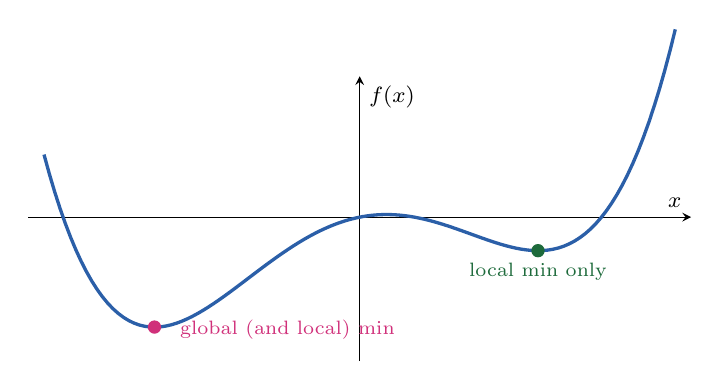
\begin{tikzpicture}
\begin{axis}[width=10cm,height=5.2cm,axis lines=middle,xmin=-2.1,xmax=2.1,ymin=-4.6,ymax=4.5,clip=false,xtick=\empty,ytick=\empty,
  xlabel={$x$},ylabel={$f(x)$},every axis label/.style={font=\footnotesize}]
\addplot[very thick,pcyan,domain=-2:2,samples=120] {x^4-3*x^2+x};
\addplot[only marks,mark=*,mark size=2.2pt,ppink] coordinates {(-1.30,-3.51)};
\addplot[only marks,mark=*,mark size=2.2pt,pgreen] coordinates {(1.13,-1.07)};
\node[ppink,font=\scriptsize,right] at (axis cs:-1.20,-3.6) {global (and local) min};
\node[pgreen,font=\scriptsize,below] at (axis cs:1.13,-1.15) {local min only};
\end{axis}
\end{tikzpicture}
\figcap{$f(x)=x^4-3x^2+x$. At $x\approx1.13$ every \emph{nearby} point is higher, so it is a local minimum, but $x\approx-1.30$ is lower still.
A downhill-walking algorithm started at $x=1.5$ gets stuck at the green point.}
\end{center}

Every global minimum is a local one, not the other way round. Algorithms only ever ``see'' the neighbourhood of where they are, which is why
we need conditions that are \emph{local} (derivatives) and then a property (convexity) that turns local into global.

\subsection{Necessary optimality conditions}

\begin{formula}[Theorem 2.7: necessary conditions, scalar case]
Let $f$ be twice continuously differentiable and $x^*$ a local minimum of $f$ over an interval $S$. Then either
\begin{itemize}
  \item $x^*$ is an \textbf{endpoint} of $S$, or
  \item $f'(x^*)=0$ \textbf{and} $f''(x^*)\ge0$.
\end{itemize}
\end{formula}

\textbf{Proof, step by step.} Assume $x^*$ is a local minimum that is not an endpoint, so we can step a little both left and right.
\begin{enumerate}
  \item \textbf{Local optimality, written down:} for all small $|\alpha|$, $f(x^*+\alpha)-f(x^*)\ge0$.
  \item \textbf{Divide by $\alpha$.} For $\alpha>0$ the quotient $\dfrac{f(x^*+\alpha)-f(x^*)}{\alpha}\ge0$; for $\alpha<0$ (dividing by a negative flips the sign) it is $\le0$.
  \item \textbf{Take the limit.} Both quotients tend to $f'(x^*)$. A limit of numbers $\ge0$ is $\ge0$, a limit of numbers $\le0$ is $\le0$. So $f'(x^*)=0$.
  \item \textbf{Exact Taylor.} $f(x^*+\alpha)-f(x^*) = \alpha f'(x^*) + \tfrac{\alpha^2}2f''(z)$ for some $z$ between $x^*$ and $x^*+\alpha$.
        The first term is $0$ by step 3.
  \item \textbf{Use optimality again:} $0\le f(x^*+\alpha)-f(x^*) = \tfrac{\alpha^2}2f''(z)$, so $f''(z)\ge0$.
  \item \textbf{Shrink $\alpha\to0$.} Then $z\to x^*$, and by continuity of $f''$, $f''(x^*)\ge0$. $\square$
\end{enumerate}

\begin{intuition}[In words]
At an interior bottom, the ground is flat ($f'=0$; if it sloped, one side would be lower) and it curves up, or at least not down ($f''\ge0$).
At an endpoint you are not allowed to step outside, so the slope can be anything.
\end{intuition}

\begin{example}[The endpoint clause matters]
$\min_{x\in[0,1]}x$: the minimizer is $x^*=0$, but $f'(0)=1\ne0$. No contradiction: $0$ is an endpoint, and stepping left (where $f$ is lower) is infeasible.
\end{example}

\begin{pitfall}[Necessary, not sufficient]
$f(x)=x^3$ at $x=0$: $f'(0)=0$ and $f''(0)=0\ge0$, so both conditions hold, yet $0$ is not a local minimum ($f(-0.1)=-0.001<0$).
The theorem only \emph{rules out} candidates; points that pass are just candidates.
\end{pitfall}

\textbf{Straightforward variations} (from the lecture):
\begin{itemize}
  \item \textbf{Maximization:} reverse the inequalities: $f'(x^*)=0$, $f''(x^*)\le0$.
  \item \textbf{Multivariate:} $\nabla f(x^*)=0$ and $\nabla^2f(x^*)\succeq0$ (PSD, Week 01).
\end{itemize}

\textbf{Why a matrix condition?} Run the scalar proof along \emph{every} line through $x^*$. Fix a direction $d$ and look at $\alpha\mapsto f(x^*+\alpha d)$:
\[ f(x^*+\alpha d)-f(x^*) = \alpha\,\nabla f(x^*)^Td + \tfrac{\alpha^2}{2}\,d^T\nabla^2f(z)\,d. \]
The scalar argument gives $\nabla f(x^*)^Td=0$ for every $d$ (so $\nabla f(x^*)=0$) and $d^T\nabla^2f(x^*)d\ge0$ for every $d$, which is exactly the definition of $\nabla^2 f(x^*)\succeq0$.

\begin{example}[A saddle point]
$f(x_1,x_2)=x_1^2-x_2^2$: $\nabla f=(2x_1,-2x_2)=0$ only at the origin, and $\nabla^2f=\Diag(2,-2)$, which is not PSD
($d=(0,1)$ gives $-2$). So the origin is \textbf{not} a local minimum: along the $x_2$-axis, $f=-x_2^2$ goes down. This shape (up in one direction,
down in another) is called a \term{saddle point}.
\end{example}

\begin{pitfall}[The lecture's ``strict'' variation, read carefully]
The notes say that for strict local minima one ``replaces the inequalities by strict ones''. That is right for the \textbf{sufficient} direction:
if $f'(x^*)=0$ and $f''(x^*)>0$, then $x^*$ is a strict local minimum. It is \textbf{not} a necessary condition:
$f(x)=x^4$ has a strict local (even global) minimum at $0$, but $f''(0)=0$, not $>0$.
\end{pitfall}

\section{Convexity}

The conditions so far are \emph{local}: they cannot tell the green point of the figure from the pink one. Convexity is the property that
makes local information global. \textbf{This week everything is in one dimension}; convexity in $\R^n$ is Chapters 7--8.

\subsection{Convex sets}

\begin{defn}[Definition 2.8: convex set]
A set $S$ is \term{convex} if for all $x,y\in S$ and all $\lambda\in[0,1]$, the point $\lambda x+(1-\lambda)y$ is also in $S$.
\end{defn}

\begin{intuition}[Reading the formula]
$\lambda x+(1-\lambda)y$ for $\lambda$ from $0$ to $1$ walks along the straight segment from $y$ (at $\lambda=0$) to $x$ (at $\lambda=1$); $\lambda=\tfrac12$ is the midpoint.
So: \hl{a set is convex if, with any two of its points, it contains the whole segment between them.} No holes, no dents.
Example: $x=4$, $y=0$, $\lambda=\tfrac14$ gives $\tfrac14\cdot4+\tfrac34\cdot0=1$, a quarter of the way from $0$ to $4$.
\end{intuition}

In one dimension the segment between $x$ and $y$ is just the interval between them, so \textbf{the convex subsets of $\R$ are exactly the intervals}:
$\{x\ge a\}$, $\{a\le x\le b\}$, $\{x\le b\}$, open or closed ends, and $\R$ itself. \src{BV \S2.1.4}

\begin{example}[Convex or not?]
$[0,5]$, $(-\infty,2)$, $\{3\}$, $\R$: convex. $[0,1]\cup[2,3]$: \textbf{not} convex, since $1$ and $2$ are in it but their midpoint $1.5$ is not.
\end{example}

\subsection{Convex functions}

\begin{defn}[Definition 2.9: convex function]
$f$ is \term{convex} over an interval $I$ if for all $x,y\in I$ and $\lambda\in[0,1]$:
\[ f(\lambda x+(1-\lambda)y)\ \le\ \lambda f(x)+(1-\lambda)f(y). \]
$f$ is \term{concave} if $-f$ is convex (reverse the inequality).
The left side needs $\lambda x+(1-\lambda)y\in I$: that is why the domain must be an interval (a convex set). \src{BV \S3.1.1}
\end{defn}

\begin{center}
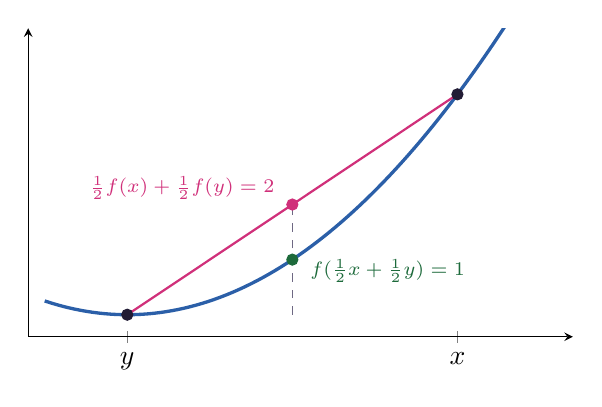
\begin{tikzpicture}
\begin{axis}[width=8.5cm,height=5.5cm,axis lines=left,xmin=-0.6,xmax=2.7,ymin=-0.4,ymax=5.2,xtick={0,2},xticklabels={$y$,$x$},ytick=\empty,
  every axis label/.style={font=\footnotesize}]
\addplot[very thick,pcyan,domain=-0.5:2.4,samples=80] {x^2};
\addplot[thick,ppink] coordinates {(0,0) (2,4)};
\addplot[only marks,mark=*,mark size=2pt,ink] coordinates {(0,0) (2,4)};
\addplot[dashed,muted] coordinates {(1,0) (1,2)};
\addplot[only marks,mark=*,mark size=2pt,pgreen] coordinates {(1,1)};
\addplot[only marks,mark=*,mark size=2pt,ppink] coordinates {(1,2)};
\node[pgreen,font=\scriptsize,right] at (axis cs:1.05,0.8) {$f(\tfrac12x+\tfrac12y)=1$};
\node[ppink,font=\scriptsize,left] at (axis cs:0.95,2.3) {$\tfrac12f(x)+\tfrac12f(y)=2$};
\end{axis}
\end{tikzpicture}
\figcap{$f(x)=x^2$, $y=0$, $x=2$, $\lambda=\tfrac12$. The left side of the definition is the graph at the midpoint (green, $1$); the right side is the chord at the midpoint
(pink, $2$). Convex: \hl{every chord lies above the graph}.}
\end{center}

\begin{intuition}[A pastry picture]
Lay a strip of Apfelstrudel dough over a bowl and pull it tight between any two points of the rim: the tight strip (the chord) never dips below
the bowl's surface (the graph). A bowl is convex; a bumpy surface (like the figure in \S2.3) is not, because a chord can pass \emph{under} a bump.
\end{intuition}

\subsection{First-order condition: above every tangent}

\begin{formula}[Theorem 2.10: first-order condition]
A continuously differentiable $f$ is convex over $I$ \textbf{if and only if}
\[ f(x)\ \ge\ f(y)+(x-y)f'(y)\qquad\text{for all } x,y\in I. \]
The right side is the tangent line at $y$, evaluated at $x$. So: \hl{a convex function lies above all of its tangent lines}. \src{BV \S3.1.3}
\end{formula}

\begin{center}
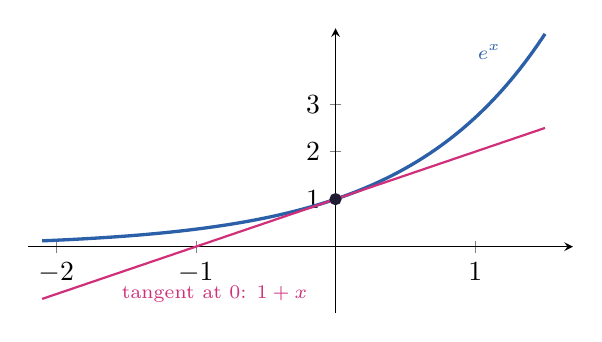
\begin{tikzpicture}
\begin{axis}[width=8.5cm,height=5.2cm,axis lines=middle,xmin=-2.2,xmax=1.7,ymin=-1.4,ymax=4.6,xtick={-2,-1,1},ytick={1,2,3},
  every axis label/.style={font=\footnotesize}]
\addplot[very thick,pcyan,domain=-2.1:1.5,samples=80] {exp(x)};
\addplot[thick,ppink,domain=-2.1:1.5] {1+x};
\addplot[only marks,mark=*,mark size=2pt,ink] coordinates {(0,1)};
\node[pcyan,font=\scriptsize] at (axis cs:1.1,4.1) {$e^x$};
\node[ppink,font=\scriptsize,right] at (axis cs:-1.6,-1.0) {tangent at $0$: $1+x$};
\end{axis}
\end{tikzpicture}
\figcap{$e^x\ge1+x$ for every $x$: the first-order condition at $y=0$ ($f(0)=1$, $f'(0)=1$).}
\end{center}

\textbf{Proof, step by step.}

\emph{($\Rightarrow$) Convex implies above tangents.}
\begin{enumerate}
  \item Fix $x\ne y$ in $I$ (if $x=y$ there is nothing to prove). Write the definition with the point $y+\lambda(x-y) = \lambda x+(1-\lambda)y$:
        $f(y+\lambda(x-y))\le\lambda f(x)+(1-\lambda)f(y)$, for $\lambda\in(0,1]$.
  \item Subtract $f(y)$ and divide by $\lambda>0$: $\dfrac{f(y+\lambda(x-y))-f(y)}{\lambda}\le f(x)-f(y)$.
  \item Write the left side as $\dfrac{f(y+\lambda(x-y))-f(y)}{\lambda(x-y)}\cdot(x-y)$. The fraction is a difference quotient with step $\lambda(x-y)$.
  \item Let $\lambda\to0$: the fraction tends to $f'(y)$. So $f'(y)(x-y)\le f(x)-f(y)$, which rearranges to the claim.
\end{enumerate}

\emph{($\Leftarrow$) Above tangents implies convex.}
\begin{enumerate}
  \item Fix $x,y$, $\lambda\in[0,1]$, and the point between them $z=\lambda x+(1-\lambda)y$.
  \item Use the tangent at $z$ twice: $f(x)\ge f(z)+(x-z)f'(z)$ and $f(y)\ge f(z)+(y-z)f'(z)$.
  \item Multiply the first by $\lambda$, the second by $1-\lambda$, and add:
        $\lambda f(x)+(1-\lambda)f(y)\ge f(z) + \big[\lambda x+(1-\lambda)y - z\big]f'(z)$.
  \item The bracket is $z-z=0$. What remains, $\lambda f(x)+(1-\lambda)f(y)\ge f(z)$, is the definition. $\square$
\end{enumerate}

\begin{intuition}[Why this is the most useful form]
The tangent line is built from information at \emph{one} point ($f(y)$, $f'(y)$), yet the inequality holds at \emph{every} $x$.
\hl{For a convex function, local information gives a global lower bound.} In particular, if $f'(y)=0$, then $f(x)\ge f(y)$ for every $x$:
a flat point of a convex function is a global minimum (Problem P15).
\end{intuition}

\subsection{Second-order condition: curving up everywhere}

\begin{formula}[Theorem 2.11: second-order condition]
A twice continuously differentiable $f$ is convex over $I$ \textbf{if and only if} $f''(x)\ge0$ for all $x\in I$. \src{BV \S3.1.4}
\end{formula}

\textbf{Proof, step by step.}
\begin{enumerate}
  \item \emph{Sufficiency.} Exact Taylor: $f(y)-f(x) = (y-x)f'(x)+\tfrac{(y-x)^2}{2}f''(z)$ for some $z$ between $x$ and $y$.
  \item If $f''\ge0$ everywhere, the last term is $\ge0$, so $f(y)\ge f(x)+(y-x)f'(x)$: the first-order condition. By Theorem 2.10, $f$ is convex.
  \item \emph{Necessity.} Suppose $f$ is convex but $f''(x)<0$ at some $x$. Since $f''$ is continuous, $f''<0$ on a small interval around $x$; pick $y\ne x$ in it.
  \item Then every $z$ between $x$ and $y$ has $f''(z)<0$, so the Taylor formula gives $f(y)<f(x)+(y-x)f'(x)$: the graph is \emph{below} a tangent.
        This contradicts Theorem 2.10. $\square$
\end{enumerate}

This is the \emph{practical} test: one derivative computation, one sign check.

\begin{center}\small
\renewcommand{\arraystretch}{1.4}
\begin{tabular}{>{\columncolor{border}}l l l l}
\thd{FUNCTION} & \cellcolor{border}\thd{DOMAIN} & \cellcolor{border}\thd{$f''(x)$} & \cellcolor{border}\thd{VERDICT}\\
\rowcolor{surface}\cellcolor{border}\color{surface}$e^x$ & $\R$ & $e^x>0$ & convex\\
\rowcolor{surface2}\cellcolor{border}\color{surface}$x^a$ & $\R_{++}=(0,\infty)$ & $a(a-1)x^{a-2}$ & convex: $a\ge1$ or $a\le0$\\ \rowcolor{surface2}\cellcolor{border} & & & concave: $0\le a\le1$\\
\rowcolor{surface}\cellcolor{border}\color{surface}$-\log x$ & $\R_{++}$ & $1/x^2>0$ & convex (so $\log x$ is concave)\\
\rowcolor{surface2}\cellcolor{border}\color{surface}$x\log x$ (negative entropy) & $\R_{++}$ & $1/x>0$ & convex\\
\end{tabular}
\end{center}

\textbf{Reading the power row.} $x^{a-2}>0$ on $\R_{++}$, so the sign of $f''$ is the sign of $a(a-1)$: positive outside $[0,1]$, negative inside.
Examples: $x^2$ ($a=2$, convex), $1/x$ ($a=-1$, $f''=2/x^3>0$, convex), $\sqrt x$ ($a=\tfrac12$, $f''=-\tfrac14x^{-3/2}<0$, concave), $x$ ($a=1$, both).
\src{BV \S3.1.5}

\begin{pitfall}[$f''\ge0$, not $f''>0$]
$f(x)=x^4$ is convex on $\R$ even though $f''(0)=0$. The condition is ``$\ge0$ everywhere''. (Conversely, one point with $f''<0$ is enough to break convexity.)
\end{pitfall}

\begin{pitfall}[The tests need derivatives; the definition does not]
$f(x)=|x|$ is convex (every chord lies on or above the V), but $f'(0)$ does not exist, so Theorems 2.10--2.11 cannot be applied at $0$. Use the
definition, or the triangle inequality: $|\lambda x+(1-\lambda)y|\le\lambda|x|+(1-\lambda)|y|$.
\end{pitfall}

\begin{pitfall}[The domain is part of the answer]
$x^3$ has $f''=6x$: convex on $[0,\infty)$, \textbf{not} convex on $\R$. Always state the interval. Similarly the power table is about $\R_{++}$ only:
$x^{-1}$ is not convex on $\R\setminus\{0\}$ (that set is not even an interval).
\end{pitfall}

\subsection{The payoff: local $=$ global}

\begin{formula}[Theorem 2.12: local $=$ global]
If $f$ is convex over an interval $I$, then every local minimum of $f$ over $I$ is a global minimum. \src{BV \S4.2.2}
\end{formula}

\textbf{Proof, step by step} (by contradiction).
\begin{enumerate}
  \item Suppose $x$ is a local minimum but not global: some $y\in I$ has $f(y)<f(x)$.
  \item Walk from $x$ toward $y$: the points $\lambda x+(1-\lambda)y$ with $\lambda$ close to $1$ are close to $x$ (and in $I$, because $I$ is an interval).
  \item Convexity: $f(\lambda x+(1-\lambda)y)\le\lambda f(x)+(1-\lambda)f(y)$.
  \item Because $f(y)<f(x)$ and $1-\lambda>0$, the right side is \emph{strictly} less than $\lambda f(x)+(1-\lambda)f(x) = f(x)$.
  \item So as $\lambda\to1$ we find points arbitrarily close to $x$ with $f<f(x)$. That contradicts $x$ being a local minimum. $\square$
\end{enumerate}

\begin{intuition}[Why the proof works]
The chord from $x$ down to the lower point $y$ starts at height $f(x)$ and goes strictly down. A convex function stays \emph{below} its chords,
so it must also go down right next to $x$. \hl{A convex function cannot hide a lower valley behind a hill}: there are no hills.
\end{intuition}

\begin{example}[Seeing it on the figure of \S2.3]
$f(x)=x^4-3x^2+x$ has a local minimum that is not global, so by Theorem 2.12 it cannot be convex. Check: $f''(x)=12x^2-6$, and $f''(0)=-6<0$. \checkmark
\end{example}

\begin{plainbox}
\textbf{Remark (from the lecture): convexity is sufficient, not necessary.} Some non-convex functions also have local $=$ global, for example
$f(x)=\sqrt{|x|}$: its only local minimum is $x=0$, which is global, but $f''(x)=-\tfrac14|x|^{-3/2}<0$ for $x\ne0$ (concave on each side).
Such functions are \emph{(strictly) quasi-convex}. Convexity is still the property we build on: it is the easiest to verify, the best understood
(no saddle points, preserved under sums), and it generalizes cleanly to $\R^n$.
\end{plainbox}

% =================================================================
\parttitle{PART B \textperiodcentered\ RECITATION 2}{Hessians and Stationary Points}
% =================================================================

\begin{plainbox}
\textbf{What the recitation does.} It drills the lecture's tools on concrete functions: compute $\nabla f$ and $\nabla^2f$, find the points where $\nabla f=0$,
and decide what kind of points they are (\S2.2 of Wiesel's notes, Exercises 2.1--2.5). Every exercise is solved below step by step.
Where the notes' solution skips a step or has a gap, a \textbf{pitfall} box says so and fills it in.
Before the exercises, \S\ref{sec:toolkit} collects the few things the recitation uses that the lecture did not state explicitly.
\end{plainbox}

\section{Toolkit for the recitation}\label{sec:toolkit}

\begin{defn}[Stationary point]
A point $x^*$ with $\nabla f(x^*)=0$ is a \term{stationary point} (also \term{critical point}). By the lecture's necessary conditions, every interior local minimum or maximum is stationary,
so the stationary points are the \emph{candidates}. A stationary point that is neither a local minimum nor a local maximum is a \term{saddle point}.
\end{defn}

\begin{defn}[Definiteness of a symmetric matrix $H$ (recap of Week 01)]
\begin{itemize}
  \item \term{PSD} ($H\succeq0$): $d^THd\ge0$ for every $d$ (all eigenvalues $\ge0$). \term{PD} ($H\succ0$): $d^THd>0$ for every $d\ne0$ (all eigenvalues $>0$).
  \item \term{NSD} / \term{ND}: the same with $\le0$ / $<0$ (i.e.\ $-H$ is PSD / PD).
  \item \term{Indefinite}: $d^THd>0$ for some $d$ and $<0$ for another (eigenvalues of both signs).
\end{itemize}
\end{defn}

\begin{formula}[The $2\times2$ shortcut]
For $H=\begin{pmatrix}a&b\\b&c\end{pmatrix}$, the eigenvalues multiply to $\det H=ac-b^2$ and add to $a+c$. So:
\begin{center}
\renewcommand{\arraystretch}{1.25}
\begin{tabular}{l l}
$\det H>0$ and $a>0$ & PD (both eigenvalues positive)\\
$\det H>0$ and $a<0$ & ND (both negative)\\
$\det H<0$ & indefinite (one of each sign)\\
$\det H=0$ & singular: PSD if $a+c\ge0$, NSD if $a+c\le0$
\end{tabular}
\end{center}
Example: $\begin{pmatrix}2&1\\1&2\end{pmatrix}$: $\det=3>0$, $a=2>0$, PD. $\begin{pmatrix}2&4\\4&2\end{pmatrix}$: $\det=-12<0$, indefinite. $\begin{pmatrix}1&1\\1&1\end{pmatrix}$: $\det=0$, trace $2$, PSD and singular.
\end{formula}

\begin{formula}[Second-derivative test at a stationary point $x^*$]
\begin{center}
\renewcommand{\arraystretch}{1.25}
\begin{tabular}{l l}
$\nabla^2f(x^*)\succ0$ (PD) & strict local minimum\\
$\nabla^2f(x^*)\prec0$ (ND) & strict local maximum\\
$\nabla^2f(x^*)$ indefinite & saddle point\\
$\nabla^2f(x^*)$ singular (PSD or NSD, not definite) & \hl{the test says nothing}: look at $f$ itself
\end{tabular}
\end{center}
\end{formula}

\textbf{Why the test works.} Exact Taylor at a stationary point: $f(x^*+d)=f(x^*)+\tfrac12d^T\nabla^2f(z)\,d$, with $z$ between $x^*$ and $x^*+d$; for small $d$, $\nabla^2f(z)\approx\nabla^2f(x^*)$.
\begin{itemize}
  \item PD: the extra term is positive in \emph{every} direction, so $f$ goes up all around: a strict minimum. (This is the lecture's ``strict'' variation, which, as the pitfall in Part A says, is a \emph{sufficient} condition.)
  \item Indefinite: the Hessian is not PSD, so by the lecture's necessary condition $x^*$ is not a local minimum; it is not NSD, so it is not a local maximum either. Hence a saddle.
  \item Singular: in a direction $d$ with $d^T\nabla^2f\,d=0$, the second-order term is zero and the behaviour is decided by higher-order terms (as with $x^3$, $x^4$, $-x^4$ in one dimension).
\end{itemize}

\begin{formula}[Rank-one matrices $aa^T$]
For a column $a\in\R^n$, $aa^T$ is the $n\times n$ matrix with entries $(aa^T)_{jk}=a_ja_k$. For every $d$:
\[ d^T(aa^T)d=(d^Ta)(a^Td)=(a^Td)^2\ \ge\ 0, \]
so \hl{$aa^T$ is always PSD}, and a positive number times $aa^T$ is PSD too. For $n\ge2$ it is singular: any $d\perp a$ gives $0$.
Example: $a=(1,2)$: $aa^T=\begin{pmatrix}1&2\\2&4\end{pmatrix}$, $\det=0$, trace $5$. \hl{Do not confuse it with $a^Ta=\norm a^2=5$, a number.}
\end{formula}

\begin{formula}[Turning ``local'' into ``global'' this week]
The second-derivative test is local. To show that a minimum is \emph{global}, use one of these:
\begin{enumerate}
  \item rewrite $f$ so a lower bound is visible (e.g.\ complete the square);
  \item a tangent-line inequality from Part A, e.g.\ $e^s\ge1+s$ for all $s$ (Theorem 2.10 for $e^x$ at $0$);
  \item a Hessian that is PSD at \emph{every} point makes $f$ convex, and then every stationary point is a global minimum (proved in Part C, Step (b)2, and in Chapters 7--8).
\end{enumerate}
\end{formula}

\section{Exercise 2.1: find and classify stationary points \lvl{$\bullet\circ\circ$}}

\textbf{Recipe.} (1) Compute $\nabla f$ and solve $\nabla f=0$. (2) Compute $\nabla^2f$ at each solution. (3) Read off the test. (4) If the test is silent, or you want ``global'', look at $f$ itself.

\subsection*{(1) $f(x,y)=x^2+y^2-2x-4y+5$}
\begin{enumerate}
  \item $\partial_xf=2x-2$, $\partial_yf=2y-4$. Both zero: $(x,y)=(1,2)$, the only stationary point.
  \item $\nabla^2f=\begin{pmatrix}2&0\\0&2\end{pmatrix}=2I$, the same at every point.
  \item $2I\succ0$: strict local minimum. Value $f(1,2)=1+4-2-8+5=0$.
  \item Global: complete the squares, $f=(x-1)^2+(y-2)^2\ge0$, with equality only at $(1,2)$.
\end{enumerate}
\textbf{Answer:} one stationary point, $(1,2)$: the unique global minimum, $f=0$. The graph is a round bowl centred at $(1,2)$.

\begin{pitfall}[``PD Hessian, so global'']
The notes say ``the Hessian is $2I\succ0$, so this is a (global) minimum''. A PD Hessian \emph{at one point} only proves a \emph{local} minimum.
Here it is global because the Hessian is PD \emph{everywhere} (tool 3), or, more simply, because of the completed square (tool 1).
\end{pitfall}

\subsection*{(2) $f(x,y)=x^3-3xy^2$}
\begin{enumerate}
  \item $\partial_xf=3x^2-3y^2$, $\partial_yf=-6xy$.
  \item Solve: $-6xy=0$ means $x=0$ or $y=0$. If $x=0$, the first equation gives $-3y^2=0$, so $y=0$. If $y=0$, it gives $3x^2=0$, so $x=0$. The only stationary point is $(0,0)$.
  \item $\nabla^2f=\begin{pmatrix}6x&-6y\\-6y&-6x\end{pmatrix}$, which is the \textbf{zero matrix} at $(0,0)$: the test is silent.
  \item Look at $f$ along the line $y=0$: $f(x,0)=x^3$. So $f(0.1,0)=0.001>0$ and $f(-0.1,0)=-0.001<0$: arbitrarily close to the origin there are higher \emph{and} lower points.
\end{enumerate}
\textbf{Answer:} $(0,0)$ is neither a minimum nor a maximum: a saddle point.

\begin{intuition}[Why it is called a monkey saddle]
In polar coordinates $x=r\cos\theta$, $y=r\sin\theta$: $f=r^3(\cos^3\theta-3\cos\theta\sin^2\theta)=r^3\cos3\theta$.
As you walk around the origin, $f$ goes up and down \emph{three} times: three valleys and three ridges. A horse saddle ($x^2-y^2$, Part A) has two valleys, for two legs;
this one has a third, for the monkey's tail.
\end{intuition}

\begin{pitfall}[Zero Hessian does not mean ``minimum'' or ``flat'']
When $\nabla^2f(x^*)=0$ (or is singular), the second-derivative test gives no information either way. You must look at $f$ directly, e.g.\ along a line, as in step 4.
\end{pitfall}

\subsection*{(3) $f(x,y)=e^{x+y}-x-y$}
\begin{enumerate}
  \item $\partial_xf=e^{x+y}-1$ and $\partial_yf=e^{x+y}-1$ (the same).
  \item Zero when $e^{x+y}=1$, i.e.\ $x+y=0$. \hl{Every point of the line $x+y=0$ is stationary}, not just one point.
  \item $\nabla^2f=e^{x+y}\begin{pmatrix}1&1\\1&1\end{pmatrix}$: $\det=0$, trace $2e^{x+y}>0$. PSD and singular, at every point: the test is silent.
  \item Look at $f$: it depends only on $s=x+y$, $f=e^s-s$. By the tangent line $e^s\ge1+s$ (tool 2), $f\ge(1+s)-s=1$, with equality only when $s=0$.
\end{enumerate}
\textbf{Answer:} every point of the line $x+y=0$ is a global minimum, with value $1$. There are infinitely many minimizers.

\begin{intuition}[A valley with a flat floor]
Along $d=(1,-1)$ the sum $x+y$ does not change, so $f$ is constant: $d^T\nabla^2f\,d=e^{x+y}(1-1)^2=0$. That zero eigenvalue is the flat floor of the valley.
Across the valley, along $(1,1)$, $f$ curves up. Picture a long tray of Kaiserschmarrn: the bottom is the same height all along its length.
\end{intuition}

\begin{center}\small
\renewcommand{\arraystretch}{1.3}
\begin{tabular}{>{\columncolor{border}}l l l l}
\thd{$f$} & \cellcolor{border}\thd{STATIONARY POINTS} & \cellcolor{border}\thd{HESSIAN THERE} & \cellcolor{border}\thd{VERDICT}\\
\rowcolor{surface}\cellcolor{border}\color{surface}$x^2+y^2-2x-4y+5$ & $(1,2)$ & $2I$, PD & global min, $0$\\
\rowcolor{surface2}\cellcolor{border}\color{surface}$x^3-3xy^2$ & $(0,0)$ & $0$, silent & saddle (monkey)\\
\rowcolor{surface}\cellcolor{border}\color{surface}$e^{x+y}-x-y$ & the line $x+y=0$ & PSD, singular & all global min, $1$\\
\end{tabular}
\end{center}

\section{Exercise 2.2: Taylor approximations \lvl{$\bullet\circ\circ$}}

\textbf{Task.} First-order approximation of $f(x,y)=e^{xy}$ around $(0,0)$, used at $(0.1,0.2)$; then the second-order expansion of $g(x)=\sin(x_1+x_2)$ around $(0,0)$.

\subsection*{$f(x,y)=e^{xy}$}
\begin{enumerate}
  \item Value: $f(0,0)=e^0=1$.
  \item Gradient (chain rule, the inner function is $xy$): $\nabla f=(ye^{xy},\ xe^{xy})$, which is $(0,0)$ at the origin.
  \item First order: $f(x,y)\approx1+(0,0)\cdot(x,y)=1$. At $(0.1,0.2)$: $\approx1$. Exact: $e^{0.02}=1.020201$. Error $0.0202$.
  \item The first order is ``too crude'' because the gradient vanishes. Go one order up. Second derivatives:
        $f_{xx}=y^2e^{xy}\to0$, $f_{yy}=x^2e^{xy}\to0$, $f_{xy}=e^{xy}+xy\,e^{xy}=(1+xy)e^{xy}\to1$ at the origin. So $\nabla^2f(0)=\begin{pmatrix}0&1\\1&0\end{pmatrix}$.
  \item Second order: $1+\tfrac12(x,y)\begin{pmatrix}0&1\\1&0\end{pmatrix}\begin{pmatrix}x\\y\end{pmatrix}=1+\tfrac12\cdot2xy=1+xy$. At $(0.1,0.2)$: $1.02$, error $0.0002$.
\end{enumerate}
\textbf{Shortcut:} $e^u\approx1+u+\tfrac{u^2}2$ with $u=xy$. The term $\tfrac{u^2}2=\tfrac{x^2y^2}2$ is of order 4, so up to order 2 only $1+xy$ remains.

\begin{pitfall}[Answer the question that was asked]
The exercise asks for the \textbf{first}-order approximation. The notes' solution says it is ``the constant 1, too crude'' and then reports $1.02$, which is the \textbf{second}-order value.
On an exam, give both: first order $f(0.1,0.2)\approx1$; second order $\approx1.02$ (exact $1.0202$).
\end{pitfall}

\subsection*{$g(x)=\sin(x_1+x_2)$}
\begin{enumerate}
  \item $g=\sin(\mathbf1^Tx)$ is an affine substitution with $a=\mathbf1=(1,1)$. By the lecture's rules: $\nabla g=\cos(\mathbf1^Tx)\,\mathbf1$ and $\nabla^2g=-\sin(\mathbf1^Tx)\,\mathbf1\mathbf1^T$.
  \item At $0$: $g(0)=0$, $\nabla g(0)=(1,1)$, $\nabla^2g(0)=-\sin(0)\,\mathbf1\mathbf1^T=0$.
  \item Second order: $g(x)\approx0+x_1+x_2+0$.
\end{enumerate}
\textbf{Answer:} $g(x)\approx x_1+x_2$; the quadratic term vanishes because $\sin''(0)=-\sin0=0$.
Check at $(0.1,0.2)$: $\sin0.3=0.29552$ vs.\ $0.3$; the error $0.0045$ is exactly the next term, $\tfrac{0.3^3}{6}=0.0045$. \checkmark

\section{Exercise 2.3: a square root of a quadratic form \lvl{$\bullet\bullet\circ$}}

\textbf{Task.} $f(x)=\sqrt{x^TQx}-b^Tx$ with $Q\succ0$ (symmetric). Compute $\nabla f$ and $\nabla^2f$, and decide whether $\nabla^2f\succeq0$.

\begin{pitfall}[The formulas need $x\ne0$; the notes do not say so]
At $x=0$, $f$ has a kink and is \textbf{not differentiable}. In one dimension, $Q=q>0$ gives $\sqrt{qx^2}=\sqrt q\,|x|$, the V-shape of $|x|$.
All formulas below hold for $x\ne0$, where $x^TQx>0$ because $Q\succ0$. Also, $\nabla(x^TQx)=2Qx$ uses that $Q$ is symmetric (Part A).
\end{pitfall}

\textbf{Gradient.}
\begin{enumerate}
  \item Name the inside: $r(x)=x^TQx$, a number. By Part A, $\nabla r=2Qx$.
  \item Outside: $\phi(r)=\sqrt r$, with $\phi'(r)=\dfrac1{2\sqrt r}$.
  \item Chain rule: $\nabla\sqrt{x^TQx}=\dfrac{1}{2\sqrt{x^TQx}}\cdot2Qx=\dfrac{Qx}{\sqrt{x^TQx}}$. And $\nabla(b^Tx)=b$.
\end{enumerate}
\[ \boxed{\ \nabla f(x)=\frac{Qx}{\sqrt{x^TQx}}-b=Qx\,(x^TQx)^{-1/2}-b\ } \]

\textbf{Hessian.} Differentiate the column $\nabla f$. The $-b$ is constant and disappears. The rest is a vector $u(x)=Qx$ times a number $c(x)=(x^TQx)^{-1/2}$.
\begin{enumerate}
  \item \textbf{Product rule for (vector) $\times$ (number):} $D[c\,u]=c\,Du+u\,(\nabla c)^T$. (Entry $(j,k)$: $\partial_k(c\,u_j)=c\,\partial_ku_j+u_j\,\partial_kc$.)
  \item $Du=Q$ (Part A, Example 2.1).
  \item $\nabla c$, by the chain rule with $\phi(r)=r^{-1/2}$ and $\phi'(r)=-\tfrac12r^{-3/2}$:
        \[ \nabla c=-\tfrac12(x^TQx)^{-3/2}\cdot2Qx=-(x^TQx)^{-3/2}\,Qx. \]
  \item Combine: $\nabla^2f=(x^TQx)^{-1/2}Q-(x^TQx)^{-3/2}\,Qx\,(Qx)^T$, and $(Qx)^T=x^TQ$ since $Q$ is symmetric.
  \item Factor out $(x^TQx)^{-3/2}$ (note $(x^TQx)^{-1/2}=(x^TQx)\cdot(x^TQx)^{-3/2}$):
\end{enumerate}
\[ \boxed{\ \nabla^2f(x)=(x^TQx)^{-3/2}\Big[(x^TQx)\,Q-Qxx^TQ\Big],\qquad x\ne0\ } \]

\begin{example}[Checks with numbers]
\begin{itemize}
  \item $n=1$, $Q=q$: the bracket is $qx^2\cdot q-q\,x\,x\,q=0$. Right: $\sqrt q|x|-bx$ is a straight line on each side of $0$, so $f''=0$.
  \item $Q=I$, $x=(1,0)$: $f=\norm x-b^Tx$ and $\nabla^2f=I-xx^T=\begin{pmatrix}0&0\\0&1\end{pmatrix}$. No curvature along $x$ (going straight out, $\norm x$ grows linearly), curvature sideways.
  \item $Q=\begin{pmatrix}2&1\\1&3\end{pmatrix}$, $x=(1,1)$: $x^TQx=7$, $Qx=(3,4)$, bracket $=7Q-\begin{pmatrix}9&12\\12&16\end{pmatrix}=\begin{pmatrix}5&-5\\-5&5\end{pmatrix}$,
        so $\nabla^2f=7^{-3/2}\begin{pmatrix}5&-5\\-5&5\end{pmatrix}\approx\begin{pmatrix}0.27&-0.27\\-0.27&0.27\end{pmatrix}$: eigenvalues $0$ and $0.54$, PSD and singular.
\end{itemize}
\end{example}

\textbf{Is the Hessian PSD? Yes.} The factor $(x^TQx)^{-3/2}$ is positive, so check the bracket.
\begin{enumerate}
  \item Write $Q=U^TU$ (possible for every $Q\succ0$: e.g.\ $U=Q^{1/2}$ from the eigendecomposition, or the Cholesky factor).
  \item For any $v$, put $y=Ux$ and $u=Uv$. Then $x^TQx=\norm y^2$, $v^TQv=\norm u^2$, $v^TQx=u^Ty$.
  \item $v^T\big[(x^TQx)Q-Qxx^TQ\big]v=(x^TQx)(v^TQv)-(v^TQx)^2=\norm y^2\norm u^2-(u^Ty)^2\ \ge\ 0$ by Cauchy--Schwarz (Week 01).
\end{enumerate}
It is never PD: $v=x$ gives $u=y$ and $\norm y^4-\norm y^4=0$. That zero is the ``no curvature along $x$'' of the examples.

\begin{pitfall}[PSD Hessian away from $0$ is not yet ``convex on $\R^n$'']
The notes remark that $f$ is convex (``a norm plus a linear function''). That is true, but a PSD Hessian on $x\ne0$ alone does not show it, because $f$ is not differentiable at $0$.
A direct proof: $\sqrt{x^TQx}=\norm{Ux}$, and by the triangle inequality $\norm{U(\lambda x+(1-\lambda)z)}\le\lambda\norm{Ux}+(1-\lambda)\norm{Uz}$; adding the linear $-b^Tx$ keeps the inequality.
\end{pitfall}

\section{Exercise 2.4: log-sum-exp and softmax \lvl{$\bullet\bullet\circ$}}

\textbf{Task.} $f(x)=\log(e^{x_1}+\dots+e^{x_n})$. Compute $\nabla f$ and interpret it.
\begin{enumerate}
  \item Inside: $S(x)=\sum_ie^{x_i}$. Only one term contains $x_j$, so $\partial S/\partial x_j=e^{x_j}$.
  \item Outside: $\log S$, derivative $1/S$.
  \item Chain rule: $\dfrac{\partial f}{\partial x_j}=\dfrac{e^{x_j}}{\sum_ie^{x_i}}$.
\end{enumerate}
\[ \boxed{\ \nabla f(x)=\frac{1}{\mathbf1^Tz}\,z,\qquad z=(e^{x_1},\dots,e^{x_n})\ } \]
\textbf{Interpretation.} The entries are positive and add up to $1$: $\nabla f$ is a probability vector, called the \term{softmax} of $x$. The largest $x_j$ gets the largest weight.

\begin{example}[With numbers]
$x=(1,2,3)$: $z=(2.718,\,7.389,\,20.086)$, sum $30.19$. $\nabla f=(0.090,\,0.245,\,0.665)$; $f=\log30.19=3.408$.
Scale up to $10x=(10,20,30)$: the softmax is $(0.000,\,0.00005,\,0.99995)$, almost exactly $e_3$, the indicator of the largest entry. That is the ``gradient'' of $\max$.
\end{example}

\begin{intuition}[How close is it to $\max$?]
$e^{\max_ix_i}\le\sum_ie^{x_i}\le n\,e^{\max_ix_i}$. Taking logs: $\ \max_ix_i\ \le\ f(x)\ \le\ \max_ix_i+\log n$.
In the example: $3\le3.408\le3+\log3=4.10$. So log-sum-exp is a smooth $\max$, off by at most $\log n$. The Hessian and convexity come in Chapter 8.
\end{intuition}

\section{Exercise 2.5: the logistic loss \lvl{$\bullet\bullet\bullet$}}

\textbf{Task.} $f(x)=\log\big(1+e^{a^Tx}\big)$, $a\in\R^n$. (1) Derivatives of $g(t)=\log(1+e^t)$ and convexity of $g$. (2) $\nabla f$, $\nabla^2f$, and $\nabla^2f\succeq0$.
(3) The empirical logistic risk $F(x)=\frac1N\sum_{i=1}^N\log\big(1+e^{-y_ia_i^Tx}\big)$, $y_i\in\{\pm1\}$, has a PSD Hessian.

\begin{defn}[Sigmoid]
$\sigma(t)=\dfrac{1}{1+e^{-t}}=\dfrac{e^t}{1+e^t}$ (multiply top and bottom by $e^t$). It increases from $0$ to $1$:
$\sigma(-2)=0.119$, $\sigma(0)=0.5$, $\sigma(2)=0.881$. Two facts used below: $1-\sigma(t)=\dfrac1{1+e^t}=\sigma(-t)$, and $\sigma'(t)=\sigma(t)\big(1-\sigma(t)\big)$.
\end{defn}
\textbf{Why $\sigma'=\sigma(1-\sigma)$:} $\sigma=(1+e^{-t})^{-1}$, so $\sigma'=(1+e^{-t})^{-2}e^{-t}=\dfrac{1}{1+e^{-t}}\cdot\dfrac{e^{-t}}{1+e^{-t}}=\sigma(t)\,(1-\sigma(t))$.

\subsection*{(1) One variable}
\begin{enumerate}
  \item $g'(t)=\dfrac{e^t}{1+e^t}=\sigma(t)$ (derivative of $\log u$ is $u'/u$, with $u=1+e^t$).
  \item $g''(t)=\sigma'(t)=\sigma(t)(1-\sigma(t))$.
  \item $0<\sigma<1$, so both factors are positive: $g''>0$ everywhere. By Theorem 2.11, $g$ is convex on $\R$.
\end{enumerate}
Check at $t=0$: $g'(0)=\tfrac12$, $g''(0)=\tfrac14$.

\subsection*{(2) The vector version}
\begin{enumerate}
  \item $f(x)=g(a^Tx)$: the affine substitution with the $1\times n$ matrix $A=a^T$.
  \item Gradient rule: $\nabla f=A^Tg'(a^Tx)=\sigma(a^Tx)\,a$.
  \item Hessian rule: $\nabla^2f=A^T\,g''(a^Tx)\,A=\sigma(a^Tx)\big(1-\sigma(a^Tx)\big)\,aa^T$.
  \item PSD: a positive number times $aa^T$, which is PSD (toolkit): $d^T\nabla^2f\,d=\sigma(1-\sigma)(a^Td)^2\ge0$.
\end{enumerate}
\[ \boxed{\ \nabla f=\sigma(a^Tx)\,a,\qquad \nabla^2f=\sigma(a^Tx)\big(1-\sigma(a^Tx)\big)\,aa^T\succeq0\ } \]
A Hessian that is PSD everywhere makes $f$ convex on $\R^n$: Part C, Step (b)2 proves this from the one-dimensional theorem.

\subsection*{(3) Many data points}
\begin{enumerate}
  \item Term $i$ is $g(c_i^Tx)$ with $c_i=-y_ia_i$. By (2), its Hessian is $\sigma(c_i^Tx)(1-\sigma(c_i^Tx))\,c_ic_i^T$, and $c_ic_i^T=y_i^2a_ia_i^T=a_ia_i^T$ because $y_i^2=1$.
  \item Each term's Hessian is PSD. A sum of PSD matrices is PSD: $d^T\big(\sum_iH_i\big)d=\sum_id^TH_id\ge0$. The factor $\frac1N>0$ keeps this.
\end{enumerate}
\textbf{Answer:} $\nabla^2F(x)=\frac1N\sum_i\sigma(c_i^Tx)(1-\sigma(c_i^Tx))\,a_ia_i^T\succeq0$. This is why \hl{logistic regression is a convex problem}.

% =================================================================
\parttitle{PART C \textperiodcentered\ EXAM CORNER}{2020 Moed B, Question 1}
% =================================================================

\begin{plainbox}
\textbf{From the exam corner of Tirgul 2} (33 points). The TA's detailed solution is in \texttt{materials/week02/}. It was checked line by line, including its numerical example, and \textbf{no errors were found};
it is reproduced below, with one shortcut added: the question is Exercise 2.5 in disguise.
\end{plainbox}

\begin{example}[The question]
For fixed vectors $w_1,\dots,w_N\in\R^n$ and $x\in\R^n$, define
\[ f(x)=\sum_{i=1}^N\log\big(1+e^{-w_i^Tx}\big). \]
(a) (25 pts) Find the Hessian of $f$. \quad (b) (8 pts) Is $f$ convex? Prove, or give a counterexample.
\end{example}

\begin{intuition}[Recognize it: Exercise 2.5 with $a=-w_i$]
Each term is $\log(1+e^{a^Tx})$ with $a=-w_i$. Exercise 2.5(2) gives its Hessian at once: $\sigma(-w_i^Tx)(1-\sigma(-w_i^Tx))\,(-w_i)(-w_i)^T$.
Since $\sigma(-t)=1-\sigma(t)$, the weight is $(1-\sigma_i)\sigma_i$, the same number, and the two minus signs cancel in $(-w_i)(-w_i)^T=w_iw_i^T$.
Below is the full derivation, as it should be written when the exam does not let you quote the exercise.
\end{intuition}

\subsection*{Before starting: who is who}
\begin{itemize}
  \item $x=(x_1,\dots,x_n)$ is the \textbf{variable}: we differentiate with respect to it. The $w_i$ are fixed data, constants for the derivative.
  \item Two indices: $i=1,\dots,N$ counts the \emph{terms} of the sum; $j,k=1,\dots,n$ count the \emph{coordinates} of $x$.
  \item Sizes: $x,w_i$ are $n\times1$; $w_i^Tx$ and $w_i^Tw_i=\norm{w_i}^2$ are numbers; \hl{$w_iw_i^T$ is an $n\times n$ matrix}.
\end{itemize}
\textbf{Plan:} (1) one variable, $h(t)=\log(1+e^{-t})$; (2) one term of the sum, coordinate by coordinate; (3) add the $N$ terms.

\subsection*{Part (a): the Hessian}
\textbf{Step 1. One variable.}
\begin{enumerate}
  \item $h'(t)=\dfrac{-e^{-t}}{1+e^{-t}}=\dfrac{-1}{e^t+1}$ (multiply top and bottom by $e^t$) $=-(1-\sigma(t))$.
  \item Write $h'(t)=-(1+e^t)^{-1}$: $h''(t)=(1+e^t)^{-2}e^t=\dfrac{e^t}{1+e^t}\cdot\dfrac{1}{1+e^t}=\sigma(t)\big(1-\sigma(t)\big)>0$.
  \item Check at $0$: $h'(0)=-\tfrac12$, $h''(0)=\tfrac14$.
\end{enumerate}
\textbf{Step 2. One term, coordinate by coordinate.} Fix $i$ and write $a=w_i$, $s=a^Tx=a_1x_1+\dots+a_nx_n$, $g(x)=h(s)$.
\begin{enumerate}
  \item Inner derivative: only $a_jx_j$ contains $x_j$, so $\partial s/\partial x_j=a_j$.
  \item First derivatives: $\dfrac{\partial g}{\partial x_j}=h'(s)\,a_j$; stacked, $\nabla g=h'(a^Tx)\,a$.
  \item Second derivatives: $a_j$ is a constant and $h'(s)$ depends on $x_k$ through $s$: $\dfrac{\partial^2g}{\partial x_k\partial x_j}=h''(s)\,a_ja_k$.
  \item As a matrix: $a_ja_k$ is entry $(j,k)$ of $aa^T$. For $n=2$: $\begin{pmatrix}a_1a_1&a_1a_2\\a_2a_1&a_2a_2\end{pmatrix}=\begin{pmatrix}a_1\\a_2\end{pmatrix}\begin{pmatrix}a_1&a_2\end{pmatrix}=aa^T$.
        So $\nabla^2g=h''(a^Tx)\,aa^T$. (The lecture's affine rule $A^T\nabla^2h\,A$ with $A=a^T$ gives this in one line.)
\end{enumerate}
\textbf{Step 3. Add up.} With $\sigma_i=\sigma(w_i^Tx)$: $\nabla f=-\sum_i(1-\sigma_i)\,w_i$, and
\[ \boxed{\ \nabla^2f(x)=\sum_{i=1}^N\sigma_i(1-\sigma_i)\,w_iw_i^T,\qquad \sigma_i=\frac{1}{1+e^{-w_i^Tx}}\ } \]
Each term has its own $\sigma_i$. Size check: $w_iw_i^T$ is $(n\times1)(1\times n)=n\times n$.

\begin{intuition}[Where did the minus sign go?]
Differentiating $\log(1+e^{-w_i^Tx})$ directly, the inner function is $-w_i^Tx$, with gradient $-w_i$. That minus appears \emph{once} in the gradient and \emph{twice} in the Hessian:
$(-w_i)(-w_i)^T=w_iw_i^T$. So the gradient has a minus sign and the Hessian does not.
\end{intuition}

\begin{example}[Check with numbers]
$n=2$, $N=3$, $w_1=(1,0)$, $w_2=(0,1)$, $w_3=(1,1)$, at $x=0$. Every $w_i^Tx=0$, so every $\sigma_i=\tfrac12$ and every weight is $\tfrac14$:
\[ \nabla^2f(0)=\tfrac14\Big[\begin{pmatrix}1&0\\0&0\end{pmatrix}+\begin{pmatrix}0&0\\0&1\end{pmatrix}+\begin{pmatrix}1&1\\1&1\end{pmatrix}\Big]=\tfrac14\begin{pmatrix}2&1\\1&2\end{pmatrix}. \]
\end{example}

\subsection*{Part (b): is $f$ convex? Yes.}
\textbf{Step 1. The Hessian is PSD at every $x$.} For any $d$: $d^Tw_iw_i^Td=(w_i^Td)^2\ge0$, so
\[ d^T\nabla^2f(x)\,d=\sum_{i=1}^N\underbrace{\sigma_i(1-\sigma_i)}_{>0}\ \underbrace{(w_i^Td)^2}_{\ge0}\ \ge\ 0. \]
\textbf{Step 2. PSD Hessian everywhere $\Rightarrow$ convex.} On the exam this is one sentence: ``by the second-order condition''. Why it is true, using only the
one-dimensional Theorem 2.11 from the lecture (restrict $f$ to a line):
\begin{enumerate}
  \item Take any $x,z\in\R^n$, $\lambda\in[0,1]$, and let $\varphi(t)=f(z+t(x-z))$. Then $\varphi(0)=f(z)$, $\varphi(1)=f(x)$, $\varphi(\lambda)=f(\lambda x+(1-\lambda)z)$.
  \item With $d=x-z$ (affine rule): $\varphi''(t)=d^T\nabla^2f(z+td)\,d\ge0$ by Step 1.
  \item So $\varphi$ is convex on $\R$ (Theorem 2.11).
  \item Since $\lambda=\lambda\cdot1+(1-\lambda)\cdot0$: $f(\lambda x+(1-\lambda)z)=\varphi(\lambda)\le\lambda\varphi(1)+(1-\lambda)\varphi(0)=\lambda f(x)+(1-\lambda)f(z)$,
        which is the definition of a convex function.
\end{enumerate}

\begin{pitfall}[Convex, but not always strictly convex]
Take $w_1=(1,1)$, $w_2=(2,2)$. Both $w_i^Tx$ depend on $x$ only through $x_1+x_2$, so $f$ is constant along $d=(1,-1)$; indeed $w_1^Td=w_2^Td=0$ gives $d^T\nabla^2f\,d=0$.
In general $f$ is strictly convex exactly when the $w_i$ span $\R^n$. Do not claim strict convexity or a unique minimizer.
\end{pitfall}

\begin{formula}[A model answer (what to write in the exam)]
(a) Let $h(t)=\log(1+e^{-t})$, $\sigma(t)=1/(1+e^{-t})$. Then $h'(t)=-(1-\sigma(t))$, $h''(t)=\sigma(t)(1-\sigma(t))$.
Term $i$ is $h(w_i^Tx)$, an affine substitution, so its Hessian is $h''(w_i^Tx)\,w_iw_i^T$. Summing:
$\nabla^2f(x)=\sum_i\sigma_i(1-\sigma_i)\,w_iw_i^T$ with $\sigma_i=\sigma(w_i^Tx)$.\\
(b) Yes. For every $d$: $d^T\nabla^2f(x)d=\sum_i\sigma_i(1-\sigma_i)(w_i^Td)^2\ge0$ since $0<\sigma_i<1$. The Hessian is PSD for every $x$, so $f$ is convex by the second-order condition.
\end{formula}

\begin{pitfall}[Where points are lost]
\begin{itemize}
  \item A minus sign in the Hessian, $-\sigma_i(1-\sigma_i)w_iw_i^T$, followed by ``$f$ is concave'' in (b).
  \item $w_i^Tw_i$ (a number) instead of $w_iw_i^T$ (an $n\times n$ matrix): check the size.
  \item One $\sigma$ for all the terms, or the sum over $i$ dropped.
  \item In (b): ``$\sigma_i(1-\sigma_i)>0$, so the Hessian is PSD'', with no word about $w_iw_i^T$. The proof needs $d^Tw_iw_i^Td=(w_i^Td)^2\ge0$.
  \item Claiming strict convexity or a unique minimizer: neither holds in general.
\end{itemize}
\end{pitfall}

% =================================================================
\parttitle{WEEK 02}{Practice Problems and Summary}
% =================================================================

\section{Practice problems with full solutions}

Try each problem before reading its solution. \lvl{$\bullet\circ\circ$} easy, \lvl{$\bullet\bullet\circ$} medium, \lvl{$\bullet\bullet\bullet$} hard.

\subsection{Derivatives}

\begin{example}[P1 \lvl{$\bullet\circ\circ$}: Jacobian and linear approximation]
$f(x_1,x_2) = (x_1x_2,\ x_1^2-x_2,\ 3x_2)$. (a) What size is $Df$? (b) Compute $Df(2,1)$. (c) Approximate $f(2.1,\,0.9)$ and compare with the exact value.

\textbf{Solution.} (a) $3$ outputs, $2$ inputs: $3\times2$.
(b) Row by row: $\nabla f_1 = (x_2,x_1)$, $\nabla f_2 = (2x_1,-1)$, $\nabla f_3 = (0,3)$. At $(2,1)$:
$Df=\begin{pmatrix}1&2\\4&-1\\0&3\end{pmatrix}$.
(c) $f(2,1)=(2,3,3)$, step $(0.1,-0.1)$: $Df\cdot(0.1,-0.1) = (0.1-0.2,\ 0.4+0.1,\ -0.3) = (-0.1,0.5,-0.3)$, so $f\approx(1.9,3.5,2.7)$.
Exact: $(2.1\cdot0.9,\ 4.41-0.9,\ 2.7) = (1.89,\ 3.51,\ 2.7)$. The third output is linear, so it is exact.
\end{example}

\begin{example}[P2 \lvl{$\bullet\circ\circ$}: gradient of a non-symmetric quadratic form]
$A=\begin{pmatrix}3&4\\0&1\end{pmatrix}$, $f(x)=x^TAx$. Compute $\nabla f(1,-1)$ in two ways, and find the symmetric matrix $S$ with $x^TSx=x^TAx$.

\textbf{Solution.} Expanded: $f=3x_1^2+4x_1x_2+x_2^2$, so $\nabla f=(6x_1+4x_2,\ 4x_1+2x_2)$, at $(1,-1)$: $(2,2)$.
Formula: $A+A^T=\begin{pmatrix}6&4\\4&2\end{pmatrix}$, times $(1,-1)$: $(2,2)$ \checkmark.
$S=\tfrac12(A+A^T)=\begin{pmatrix}3&2\\2&1\end{pmatrix}$, and then $\nabla f = 2Sx$.
\end{example}

\begin{example}[P3 \lvl{$\bullet\bullet\circ$}: least squares by hand]
$A=\begin{pmatrix}1&0\\0&1\\1&1\end{pmatrix}$, $b=(1,1,0)$, $h(x)=\norm{Ax-b}^2$. Compute $\nabla h$ and $\nabla^2h$, and find the stationary point. Is it a minimum?

\textbf{Solution.} By the affine chain rules: $\nabla h=2A^T(Ax-b)$, $\nabla^2h=2A^TA$.
$A^TA=\begin{pmatrix}2&1\\1&2\end{pmatrix}$, $A^Tb=(1,1)$. Setting $\nabla h=0$: $A^TAx=A^Tb$, i.e.\ $2x_1+x_2=1$, $x_1+2x_2=1$, so $x^*=(\tfrac13,\tfrac13)$.
The Hessian $2A^TA$ has eigenvalues $6,2>0$ (Week 01 example), so it is PD: the necessary conditions hold, and (Chapters 7--8) this is the global minimum.
Value: $Ax^*-b = (-\tfrac23,-\tfrac23,\tfrac23)$, $h(x^*)=\tfrac43$.
\end{example}

\begin{example}[P4 \lvl{$\bullet\bullet\circ$}: an exponential of a linear function]
$h(x)=e^{a^Tx}$ with $a\in\R^n$. Find $\nabla h$ and $\nabla^2h$. Show $\nabla^2h\succeq0$. Evaluate both at $x=0$ for $a=(1,2)$.

\textbf{Solution.} $h=g(a^Tx)$ with $g(t)=e^t$, and $a^Tx$ is affine with ``$A$'' $=a^T$ ($1\times n$). So $\nabla h=a\,g'(a^Tx)=e^{a^Tx}a$ and
$\nabla^2h = a\,g''(a^Tx)\,a^T = e^{a^Tx}aa^T$. For any $v$: $v^T(e^{a^Tx}aa^T)v = e^{a^Tx}(a^Tv)^2\ge0$.
At $x=0$: $\nabla h=(1,2)$, $\nabla^2h=\begin{pmatrix}1&2\\2&4\end{pmatrix}$ (PSD, singular: $\det=0$).
\end{example}

\begin{example}[P5 \lvl{$\bullet\bullet\circ$}: second-order Taylor]
$f(x_1,x_2)=e^{x_1}\cos x_2$. Write the second-order expansion around $(0,0)$ and use it to approximate $f(0.1,0.2)$.

\textbf{Solution.} $f(0)=1$. $\nabla f=(e^{x_1}\cos x_2,\ -e^{x_1}\sin x_2)=(1,0)$ at $0$.
\[ \nabla^2f=\begin{pmatrix}e^{x_1}\cos x_2&-e^{x_1}\sin x_2\\-e^{x_1}\sin x_2&-e^{x_1}\cos x_2\end{pmatrix}=\begin{pmatrix}1&0\\0&-1\end{pmatrix}\ \text{at } 0. \]
So $f\approx1+x_1+\tfrac12(x_1^2-x_2^2)$. At $(0.1,0.2)$: $1+0.1+\tfrac12(0.01-0.04)=1.085$. Exact: $e^{0.1}\cos0.2\approx1.10517\cdot0.98007\approx1.0832$.
\end{example}

\subsection{Optimality}

\begin{example}[P6 \lvl{$\bullet\circ\circ$}: does a minimizer exist?]
(a) $\min_{x\ge0}e^{-x}$; (b) $\min_{x\in[-1,1]}x^2$; (c) $\min_{x\in\R}x^3$; (d) $\min_{x>0}\,(x+1/x)$.

\textbf{Solution.} (a) No: $e^{-x}\to0$ but never reaches $0$ (infimum $0$). (b) Yes, $x^*=0$. (c) No: unbounded below.
(d) Yes: $f'=1-1/x^2=0$ at $x=1$; $f''=2/x^3>0$ on $x>0$, so $f$ is convex there and $x^*=1$ is global (Theorem 2.12), $f(1)=2$.
\end{example}

\begin{example}[P7 \lvl{$\bullet\bullet\circ$}: interior points and endpoints]
Find all local and global minima and maxima of $f(x)=x^3-3x$ on $[-3,3]$.

\textbf{Solution.}
\begin{enumerate}
  \item Interior candidates: $f'=3x^2-3=0$ at $x=\pm1$. $f''=6x$: $f''(1)=6>0$, local min, $f(1)=-2$; $f''(-1)=-6<0$, local max, $f(-1)=2$.
  \item Endpoints: $f(-3)=-27+9=-18$, $f(3)=27-9=18$.
  \item Compare: global min at the endpoint $x=-3$ (value $-18$), global max at $x=3$ ($18$).
\end{enumerate}
Note $f'(-3)=24\ne0$ at the global minimum: allowed, by the endpoint clause of Theorem 2.7. And $x=1$ is local but not global, so $f$ is not convex on
$[-3,3]$ (indeed $f''<0$ for $x<0$).
\end{example}

\begin{example}[P8 \lvl{$\bullet\bullet\circ$}: classify the stationary points]
(a) $f=x_1^2+4x_1x_2+x_2^2$. (b) $f=x_1^2+x_1x_2+x_2^2-3x_1$.

\textbf{Solution.} (a) $\nabla f=(2x_1+4x_2,\ 4x_1+2x_2)=0$ only at $0$. $\nabla^2f=\begin{pmatrix}2&4\\4&2\end{pmatrix}$, eigenvalues $6$ and $-2$: not PSD, so $0$ is a
saddle, not a minimum. Along $d=(1,-1)$: $f(t,-t)=t^2-4t^2+t^2=-2t^2<0$.
(b) $\nabla f=(2x_1+x_2-3,\ x_1+2x_2)=0$: from the second, $x_1=-2x_2$; then $-3x_2=3$, so $x^*=(2,-1)$.
$\nabla^2f=\begin{pmatrix}2&1\\1&2\end{pmatrix}\succ0$. The necessary conditions hold; $f(2,-1)=4-2+1-6=-3$.
\end{example}

\begin{example}[P9 \lvl{$\bullet\circ\circ$}: necessary is not sufficient]
For each $f$, check whether $x=0$ satisfies $f'(0)=0$, $f''(0)\ge0$, and whether it is a local minimum: (a) $x^4$; (b) $-x^4$; (c) $x^3$; (d) $x^2$.

\textbf{Solution.} All four have $f'(0)=0$. $f''(0)$: (a) $0$, (b) $0$, (c) $0$, (d) $2$. So all four \emph{pass} the necessary test.
Local min? (a) yes, (b) no (it is a max), (c) no, (d) yes. The test cannot separate (a) from (b) and (c).
\end{example}

\subsection{Convexity}

\begin{example}[P10 \lvl{$\bullet\circ\circ$}: convex sets in $\R$]
Which are convex: (a) $[2,7]$; (b) $\{x: x^2\le4\}$; (c) $\{x: x^2\ge4\}$; (d) the integers $\mathbb Z$; (e) $\{x:|x-1|<3\}$?

\textbf{Solution.} (a) yes. (b) $=[-2,2]$, yes. (c) $=(-\infty,-2]\cup[2,\infty)$, no: $-2$ and $2$ are in it, their midpoint $0$ is not.
(d) no: $0,1\in\mathbb Z$ but $\tfrac12\notin\mathbb Z$. (e) $=(-2,4)$, yes.
\end{example}

\begin{example}[P11 \lvl{$\bullet\bullet\circ$}: convexity of $x^2$ from the definition]
Prove that $f(x)=x^2$ is convex on $\R$ using only Definition 2.9 (no derivatives).

\textbf{Solution.} Compute right side minus left side:
\[ \lambda x^2+(1-\lambda)y^2-(\lambda x+(1-\lambda)y)^2 = \lambda(1-\lambda)x^2+\lambda(1-\lambda)y^2-2\lambda(1-\lambda)xy = \lambda(1-\lambda)(x-y)^2\ge0, \]
using $\lambda-\lambda^2=\lambda(1-\lambda)$ and $(1-\lambda)-(1-\lambda)^2=\lambda(1-\lambda)$. Both factors are $\ge0$ for $\lambda\in[0,1]$. Check with the figure:
$\lambda=\tfrac12$, $x=2$, $y=0$: $\tfrac14\cdot4=1 = 2-1$. \checkmark
\end{example}

\begin{example}[P12 \lvl{$\bullet\circ\circ$}: the second-order test]
Convex, concave, or neither, on the given domain? (a) $x^2+1/x$ on $\R_{++}$; (b) $\sqrt x$ on $\R_{++}$; (c) $e^{x^2}$ on $\R$; (d) $x^3$ on $\R$; (e) $\log x - x^2$ on $\R_{++}$; (f) $\cos x$ on $[-\tfrac\pi2,\tfrac\pi2]$.

\textbf{Solution.}
(a) $f''=2+2/x^3>0$: convex.
(b) $f''=-\tfrac14x^{-3/2}<0$: concave.
(c) $f'=2xe^{x^2}$, $f''=(2+4x^2)e^{x^2}>0$: convex.
(d) $f''=6x$ changes sign: neither.
(e) $f''=-1/x^2-2<0$: concave.
(f) $f''=-\cos x\le0$ there: concave.
\end{example}

\begin{example}[P13 \lvl{$\bullet\bullet\circ$}: an inequality from a tangent line]
Use the first-order condition for $f(x)=-\log x$ at $y=1$ to prove $\log x\le x-1$ for all $x>0$. When is it an equality?

\textbf{Solution.} $f$ is convex on $\R_{++}$ (table), $f(1)=0$, $f'(1)=-1/1=-1$. Theorem 2.10: $-\log x\ge0+(x-1)(-1)=1-x$, i.e.\ $\log x\le x-1$.
Equality at $x=1$ (touching point). Numbers: $x=2$: $\log2\approx0.693\le1$; $x=0.5$: $-0.693\le-0.5$. \checkmark
\end{example}

\begin{example}[P14 \lvl{$\bullet\bullet\circ$}: two valleys]
$f(x)=x^4-2x^2$. Find all local minima and maxima. Is $f$ convex on $\R$? On $[1,\infty)$? Draw the chord that breaks convexity.

\textbf{Solution.} $f'=4x(x^2-1)=0$ at $0,\pm1$. $f''=12x^2-4$: $f''(0)=-4$, local max ($f=0$); $f''(\pm1)=8$, local minima ($f=-1$, both global).
Not convex on $\R$: $f''(0)<0$. Chord from $-1$ to $1$: at the midpoint, chord height $\tfrac12(-1)+\tfrac12(-1)=-1$, but $f(0)=0>-1$: the graph is above the chord.
On $[1,\infty)$: $f''\ge12-4=8>0$, convex. (In fact $f''\ge0$ exactly when $|x|\ge1/\sqrt3$.)
\end{example}

\begin{example}[P15 \lvl{$\bullet\bullet\bullet$}: a flat point of a convex function is a global minimum]
Let $f$ be differentiable and convex on an interval $I$, and $f'(x^*)=0$ for an interior $x^*$. Prove $x^*$ is a global minimum, without using Theorem 2.12.

\textbf{Solution.} Theorem 2.10 with $y=x^*$: $f(x)\ge f(x^*)+(x-x^*)\cdot0=f(x^*)$ for all $x\in I$. That is the definition of a global minimum.
\emph{So for convex $f$ the necessary condition $f'=0$ is also sufficient}, in contrast with P9 ($x^3$, $-x^4$ are not convex).
\end{example}

\begin{example}[P16 \lvl{$\bullet\bullet\bullet$}: sums and scalings preserve convexity]
(a) If $f,g$ are convex on $I$ and $\alpha,\beta\ge0$, show $\alpha f+\beta g$ is convex using the definition.
(b) Use (a) and the table to show $h(x)=3e^x-2\log x+x\log x$ is convex on $\R_{++}$, and check with $h''$.
(c) Is $f-g$ convex in general?

\textbf{Solution.} (a) Write $m=\lambda x+(1-\lambda)y$. Then
$\alpha f(m)+\beta g(m)\le\alpha[\lambda f(x)+(1-\lambda)f(y)]+\beta[\lambda g(x)+(1-\lambda)g(y)] = \lambda(\alpha f+\beta g)(x)+(1-\lambda)(\alpha f+\beta g)(y)$.
The inequality needs $\alpha,\beta\ge0$ (multiplying by a negative number would flip it).
(b) $3e^x$, $2(-\log x)$ and $x\log x$ are nonnegative multiples of convex functions. Check: $h''=3e^x+2/x^2+1/x>0$. \checkmark
(c) No: $f=x^2$, $g=2x^2$ are convex, but $f-g=-x^2$ is concave.
\end{example}

\section{Cheat sheet}

\begin{formula}[Week 02 on one page]
\begin{itemize}
  \item \textbf{Jacobian} $Df(x)$: $m\times n$, $[Df]_{ij}=\partial f_i/\partial x_j$. $f(z)\approx f(x)+Df(x)(z-x)$. $D(Ax)=A$.
  \item \textbf{Gradient} ($m=1$): $\nabla f=(Df)^T$, a column. $f(z)\approx f(x)+\nabla f(x)^T(z-x)$; points uphill.
        $\nabla(a^Tx)=a$, $\nabla(x^TAx)=(A+A^T)x$ ($=2Ax$ if symmetric).
  \item \textbf{Chain rule}: $D[g(f(x))]=Dg(f(x))\,Df(x)$. Affine: $\nabla g(Ax+b)=A^T\nabla g(\cdot)$, $\nabla^2=A^T\nabla^2g(\cdot)A$.
        Least squares: $\nabla\norm{Ax-b}^2=2A^T(Ax-b)$, $\nabla^2=2A^TA$.
  \item \textbf{Hessian}: $[\nabla^2f]_{ij}=\partial^2f/\partial x_i\partial x_j$, symmetric. Taylor:
        $f(y)\approx f(x)+\nabla f^T(y-x)+\tfrac12(y-x)^T\nabla^2f(x)(y-x)$; exact with $\nabla^2f(z)$, $z$ on the segment.
  \item \textbf{Problem} $\min_{x\in S}f$: objective, feasible set. A minimizer may not exist ($\min x$, $\min e^x$).
        Global: $f(x^*)\le f(x)\ \forall x\in S$. Local: same, only for $\norm{x-x^*}<\epsilon$.
  \item \textbf{Necessary conditions} (local min, interior): $f'=0,\ f''\ge0$; in $\R^n$: $\nabla f=0,\ \nabla^2f\succeq0$. At an endpoint anything goes.
        Not sufficient ($x^3$). $f'=0,\ f''>0$ is sufficient for a strict local min.
  \item \textbf{Convex set}: contains every segment; in $\R$, exactly the intervals.
  \item \textbf{Convex function}: $f(\lambda x+(1-\lambda)y)\le\lambda f(x)+(1-\lambda)f(y)$ (chord above graph). Concave: $-f$ convex.
  \item \textbf{Tests} (1-D): $f(x)\ge f(y)+(x-y)f'(y)$ (above tangents) $\iff$ convex $\iff$ $f''\ge0$ on $I$.
  \item \textbf{Examples} on $\R_{++}$: $e^x$ (on $\R$), $x^a$ ($a\ge1$ or $a\le0$), $-\log x$, $x\log x$ convex; $x^a$ ($0\le a\le1$), $\log x$ concave.
  \item \textbf{Local $=$ global} for convex $f$; and for convex differentiable $f$, $f'(x^*)=0\Rightarrow$ global min.
\end{itemize}
\end{formula}

\begin{formula}[Recitation 2 and the exam on one page]
\begin{itemize}
  \item \textbf{Classify} a stationary point ($\nabla f=0$) by $\nabla^2f$: PD $\to$ strict local min; ND $\to$ strict local max; indefinite $\to$ saddle; singular $\to$ silent, look at $f$ (e.g.\ along a line).
  \item $2\times2$: $\det>0,a>0$ PD; $\det>0,a<0$ ND; $\det<0$ indefinite; $\det=0$ singular.
  \item Global: complete the square; $e^s\ge1+s$; Hessian PSD \emph{everywhere} $\Rightarrow$ convex $\Rightarrow$ every stationary point is global.
  \item $aa^T$: $n\times n$, entries $a_ja_k$, PSD since $d^Taa^Td=(a^Td)^2$. Not $a^Ta=\norm a^2$.
  \item $\nabla\sqrt{x^TQx}=Qx/\sqrt{x^TQx}$, $\nabla^2=(x^TQx)^{-3/2}[(x^TQx)Q-Qxx^TQ]\succeq0$ (Cauchy--Schwarz), only for $x\ne0$.
  \item Log-sum-exp: $\nabla=$ softmax $=z/\mathbf1^Tz$, $z_i=e^{x_i}$; $\max_ix_i\le f\le\max_ix_i+\log n$.
  \item $\sigma(t)=1/(1+e^{-t})$, $1-\sigma(t)=\sigma(-t)$, $\sigma'=\sigma(1-\sigma)$. $\log(1+e^t)$: $'=\sigma$, $''=\sigma(1-\sigma)$. $\log(1+e^{-t})$: $'=-(1-\sigma)$, $''=\sigma(1-\sigma)$.
  \item Affine: $f=g(a^Tx)\Rightarrow\nabla f=g'(a^Tx)a$, $\nabla^2f=g''(a^Tx)aa^T$. Exam: $\nabla^2\sum_i\log(1+e^{-w_i^Tx})=\sum_i\sigma_i(1-\sigma_i)w_iw_i^T\succeq0$: convex, strictly iff the $w_i$ span $\R^n$.
  \item PSD Hessian everywhere $\Rightarrow$ convex: restrict to a line, $\varphi(t)=f(z+td)$, $\varphi''=d^T\nabla^2f\,d\ge0$.
\end{itemize}
\end{formula}

\end{document}
